\setcounter{chapter}{6} %this gives Chapter 7
\chapter{Heating rate and ion shuttle}
\label{chapter:heating}

This chapter describes two studies. The first is to characterize the optical system at the trap, leading to experiments measuring the heating rate of the Sandia trap. The second involves experiments of shuttling the ion along	 the trap axis, to prepare the ground for multiple ion manipulation.  

\section{Optical system characterization}

To interpret the heating rate experiments presented in the next section, a number of parameters of the experimental setup had to be measured. These parameters characterize the laser beams (laser intensity calibration, polarization angle and linewidth for both 397\nm\, and 866\nm\, laser beams), the imaging system (optical detection efficiency, PMT dark counts), and magnetic field coil (magnetic field). In this section the measurements of these parameters are discussed.

We are able to measure beam power with the use of a photodiode or powermeter, and for laser intensity calibration we have to know the spotsize of the laser beam at the position of the ion. If the Gaussian beam spot sizes are measured ($w_H$ and $w_V$ for the horizontal and vertical direction, respectively), the laser intensity  at the beam centre is
\be
I = \frac{\pi}{2 w_H w_V} P
\label{eq:laserint}
\ee
where $P$ is the power. To estimate the laser intensity at the ion, an optical set-up similar to that illuminating the ion was used, but with a CCD camera at the ion's position. This allowed the beam profile to be measured directly. Our aim was to maximize the available 397\nm\, beam intensity. The measured spotsize for the 397\nm\, beam at its focal point (the ion's expected position) in our optical setup was
\be
w_H w_V = 87\um \times 25\um = 2175\um^2. 
\ee
The 866\nm\, beam was not measured this way.

The laser linewidth is considered to be of the order of 1\MHz\, for both beams, based on knowledge of the same types of laser used in another experiment. The polarization angle to the magnetic field is set by a PBS cube and a $\lambda/2$ plate in each beam's path. 

The calculation of the estimated optical detection efficiency is shown in Table~\ref{tab:efficiency} on page \pageref{tab:efficiency}, and has the result of $\eta = 0.16(3)\%$. The PMT dark count rate was measured to be of the order of 25\Hz \cite{Myerson2007}. The magnetic field generated by the field coil as a function of drive current was measured using a hand-held gauss-meter to be approximately $10\G/\A$. 

All of the aforementioned parameters can also be deduced from fitting theoretical curves calculated using Bloch equations to experimentally recorded fluorescence spectra. Checking the numbers in this way is particularly important because in practice all our experiments are of this type and we must be satisfied that we can interpret the data reliably.

The experiment was conducted as follows. A single ion was loaded into the trap. Micromotion compensation was performed using the RF-photon correlation as described earlier. Using the Doppler-cooling beams (397\nm\, and 866\nm), the 397\nm\, laser detuning was then scanned from red to blue detuning over the resonance of the transition and the fluorescence was recorded (see Figure~\ref{fig:satexamplefit}). When the 397nm laser is blue detuned, the ion is heated instead of cooled, and quickly gains enough energy to leave the trap. Thus the fluorescence on the blue side of the transition drops to the background level and the ion is lost. This background level is also recorded for the given laser power. A new ion is loaded, and the whole procedure repeated at a different laser power. During this experiment the 866\nm\, laser power and detuning, the magnetic field and the polarization angle of the laser beams were nominally kept at a constant value. 

The recorded spectra were fitted with theoretical fluorescence profiles calculated using Bloch-equations including the effect of micromotion. Table~\ref{tab:satfitparams} lists the fitted experimental parameters. Certain parameters had fixed values for all the scans (denoted as ``Constant'' in Table~\ref{tab:satfitparams}) such as the laser beam polarization angle and the laser linewidth. The background count was measured for every scan and thus been fixed for the fit.

To reduce the number of variables, some of the parameters were used as a single variable for all different laser powers (denoted as ``Joint fit''). These included 866\nm\, laser power, the magnetic field, the optical detection efficiency. Before every scan, the micromotion was compensated, thus the micromotion maximum velocity (as a parameter describing the residual micromotion after the compensation) can be assumed to be the same in every scan. The inclusion of micromotion had the largest effect on the fits of the lowest laser intensities, but appeared to improve the fits in general.

The 397\nm\, laser intensity is also listed as one of the ``Joint fit'' parameters. To explain this, Figure~\ref{fig:397satbg} shows the measured background counts as a function of laser power. The background scatter is proportional to the laser intensity in the area of the ion and it shows very good proportionality to the measured powers. It is then justifiable to fix the intensities of the different scans in relation to each other using their measured background scatter (above the dark counts of zero laser power). We then have a single scaling factor describing the laser powers for all the scans, given their background counts. Thus the unit of fitted laser intensity is $I_S / bg$ = ``397\nm\, saturation intensity / background count above dark counts in 100\ms\, measurement'', where the saturation intensity is defined as in Equation~\ref{eq:satintdef}. The 397\nm\, resonance position and 866\nm\, laser detuning were floated as they were noticed to change on a time scale of order minutes in previous experiments.

This arrangement resulted in 37 fitting parameters for the 16 recorded scans. An example of a fitted fluorescence profile is shown in Figure~\ref{fig:satexamplefit}. The part of the recorded fluorescence used to determine the background counts is truncated in the figure. The background was averaged over $\approx$300 points (100\ms/point) in each scan. The residuals from the best fit are also plotted.

\begin{table}[h!t]
\begin{center}
\begin{tabular}{|l|c|c|c|}
\hline
\textbf{Parameter} & \textbf{Constant} & \textbf{Joint fit}& \textbf{Individual fit}\\ 
\hline
397nm laser intensity,  $I_{397}$ &  & $0.0172 I_{S,397} / bg$ &  \\
\hline
397nm resonance position, $\Delta_{397}$&  &  & X  \\
\hline
866nm laser intensity,  $I_{866}$ &  & $295 I_{S,866}$ &  \\
\hline
866nm laser detuning,  $\Delta_{866}$ &  &  & X \\
\hline
397nm laser linewidth, $g_{397}$ & 1\MHz&  &  \\
\hline
866nm laser linewidth,  $g_{866}$ & 1\MHz &  &  \\
\hline
397nm laser polarization angle,  $\phi_{397}$ & $\pi/4$ &  &  \\
\hline
866nm laser polarization angle,  $\phi_{866}$ & $\pi/2$ &  &  \\
\hline
Magnetic field,  B &  & 3.6\G &  \\
\hline
Micromotion maximum velocity,  $v_{max}$ &  & 6\mps &  \\
\hline
Optical detection efficiency,  $\eta$ &  & 0.155\% &  \\
\hline
Background count,  $bg$ & measured &  &  \\
\hline
\end{tabular}
\end{center}
\caption{List of parameters in the fit of the recorded fluorescence spectra. Parameters noted as ``constant'' are set the same for all different spectra. ``Joint'' fit parameters are fitted as single variables for all spectra. ``Individual'' fit parameters are fitted separately for all spectra. Fitted parameter values are shown for ``Joint'' fit. Background counts are measured for every scan. The unit of 397\nm\, laser intensity is $I_{S,397} / bg$ = ``397\nm\, saturation intensity / background count over dark counts in 100\ms\, measurement'' (see text). The unit of 866nm laser intensity the 866\nm\, saturation intensity $I_{S,866}$. The saturation intensities are defined in Equation~\ref{eq:satintdef}. }
\label{tab:satfitparams}
\end{table}



In Figure~\ref{fig:397saturation} the maximum fluorescence points are plotted as a function of measured laser power. The points are scattered because of the different 866\nm\, laser detunings of the scans. The 866\nm\, laser detuning was stable to approximately $\pm 4\MHz$, which is generally not a problem. For illustration, a trend is plotted when a single common 866nm laser detuning (the average of the fitted values) is assumed and all other fitted parameters were kept the same.

The 397\nm\, resonance position was also stable to about $\pm 4\MHz$ which is sufficient for our purposes. However, the resonance position appears to have an approx. 28 minutes periodicity, see Figure~\ref{fig:397resonancepos}. This periodicity is close to the observed period of the air-conditioning system. The likely cause of this is temperature change in the piezo driver that was used to scan the laser frequency by the locking cavity. The piezo driver was placed on an area of airflow and its temperature is likely to be affected by the on/off cycle of the air-conditioning. This effect was discovered only during the data analysis, and does not have a substantial effect on the results.


Using the fitted laser intensities and the laser power at the position of the ion, the 397\nm\, beam spot-size can be determined. The laser power during the scans was measured after the beam leaves the vacuum chamber, and goes through an IR mirror and an IR filter. To be able to relate the measured laser power to the power in the trapping region, measurements were made for a number of powers at two alternative positions along the beampath: before entering the vacuum chamber, and immediately after leaving it. Table~\ref{tab:relativepower} summarizes the results of relative powers at the different positions. The power measured after the vacuum chamber is a factor of 0.615 lower than the one measured before the input window. Taking the average between the powers before and after the vacuum chamber, the relative laser power at the ion's position can be estimated as 0.96, thus the conversion factor from measured laser power to power at the ion is $\frac{0.96}{0.615}$.

The laser intensity is calculated from the laser power as
\be
I_{397} = \frac{\pi}{2 w_H w_V} P_{397,\mbox{ion}} = 
\frac{\pi}{2 w_H w_V} \frac{0.96}{0.615} P_{397,\mbox{measured}}
\label{eq:intpower397}
\ee
where $ P_{397,\mbox{measured}}$ and $ P_{397,\mbox{ion}}$ are the measured laser power and estimated power power at the ion's position, respectively, $w_H$,$w_V$ are horizontal and vertical beam parameters, and their product is estimated by the fitting procedure. The fluorescence fit and laser power measurement yields
\be
w_H w_V = 2156\um^2
\ee
which is close to the measured value $w_H w_V = 2175\um^2$; thus, the beam is likely to be focused to at the ion's position with good precision.

The beam size of the 866\nm\, beam can be similarly estimated from the fitted intensity and measured power. In the case of the 866\nm\, beam the power was measured only before the vacuum chamber and the 0.96 factor obtained previously is used to extrapolate to the position of the ion. The measured laser power $P_{866,\mbox{measured}} = 1.96\mW$. Using a similar expression to Equation~\ref{eq:intpower397} we obtain
\be
w_H w_V = 46900\um^2.
\ee

The magnetic field coil was operated at $I_{coil} = 379\mA$, thus the fitted magnetic field of 3.6\G\, is in reasonable agreement with the expected value of 3.79\G. 
The maximum ion velocity of the micromotion is fitted as $v_{max} = 6\mps$. In case of optimal cooling, the ion's motion is entirely due to the effect of the RF field oscillating at $\Omega_{RF} = 2\pi \times 27.25\MHz$. Taking the 45\degree\, viewing angle into account, the $v_{max}$ corresponds to an oscillation with amplitude $A \approx 50 \nm$.
The detection efficiency was fitted as 0.155\%, in agreement with the calculated 0.16(3)\%.

The fact that the experimental parameters derived from the fits are consistent with the results of separate measurements gives confidence in the general approach. 

\begin{table}[t]
 \begin{center}
% use packages: array
\begin{tabular}{|c|c|}
\hline
\textbf{Power measurement position} & \textbf{Relative power} \\ 
\hline
Before input window 			& 1 \\ 
After output before mirror/filter 	& 0.92 \\ 
After output window and mirror/filter 	& 0.615 \\
%After output window and mirror/filter 	& 0.68 \\
\hline
\end{tabular}
\end{center}
\caption{Laser power of the 397\nm\, beam measured at different positions along the beam path.}
\label{tab:relativepower}
\end{table}


\begin{figure}[t]
\centering
%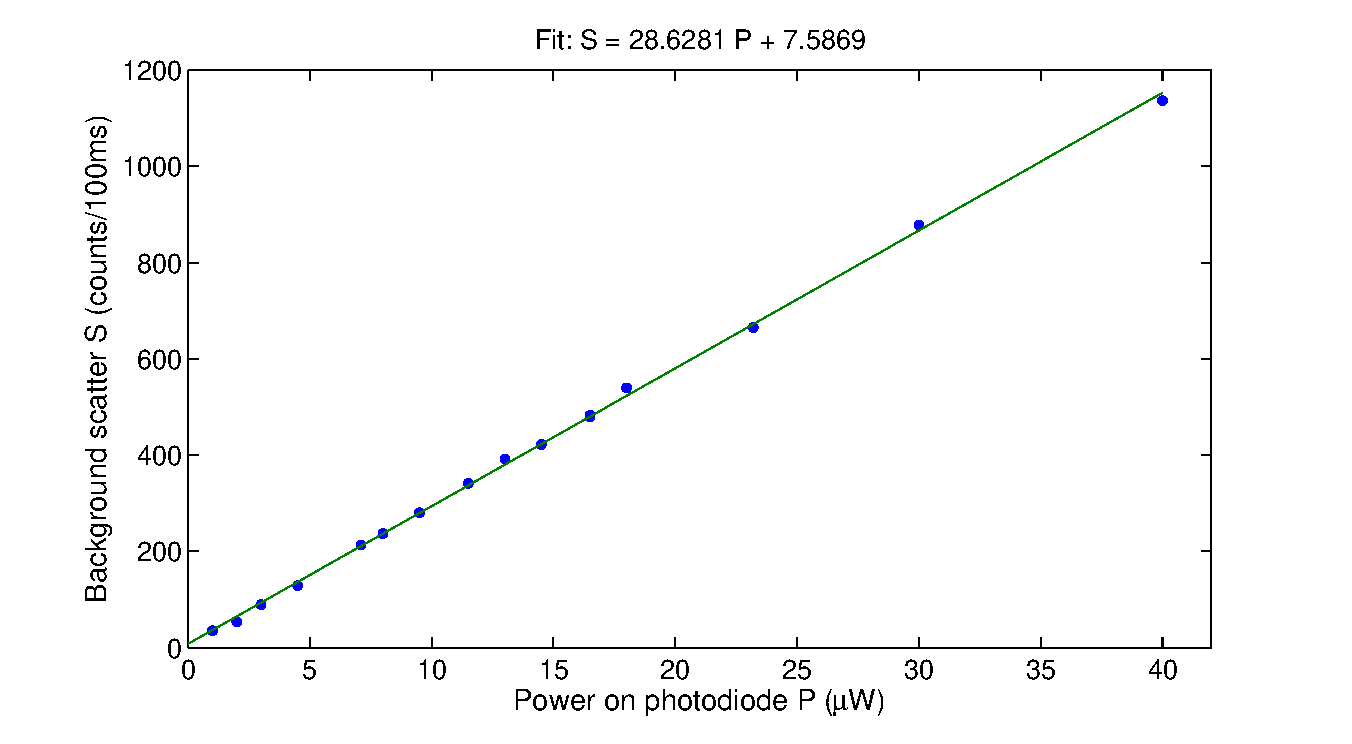
\includegraphics[width=12.5cm]{chapter7/saturation/background_v2}
\includegraphics{chapter7/saturation/background_v4}
\caption[Background counts as function of laser power]{Measured background count rate as a function of measured laser power on the photodiode. The intercept of the fit (7.6 counts) provides an estimate of the dark counts of the PMT.}
\label{fig:397satbg}
\end{figure} 

\begin{figure}[h!t]
\centering
%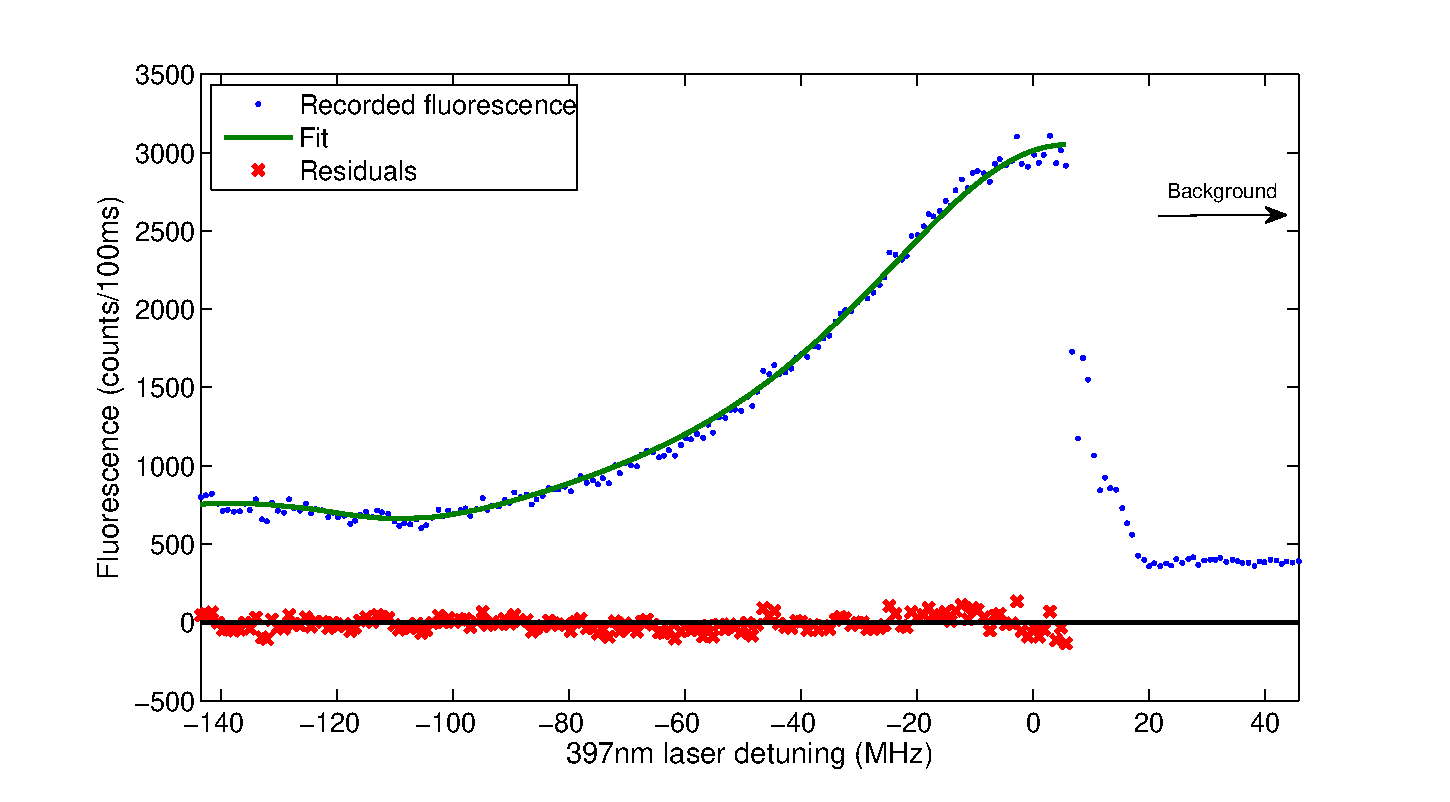
\includegraphics[width=12.5cm]{chapter7/saturation/397satfit10_v3}
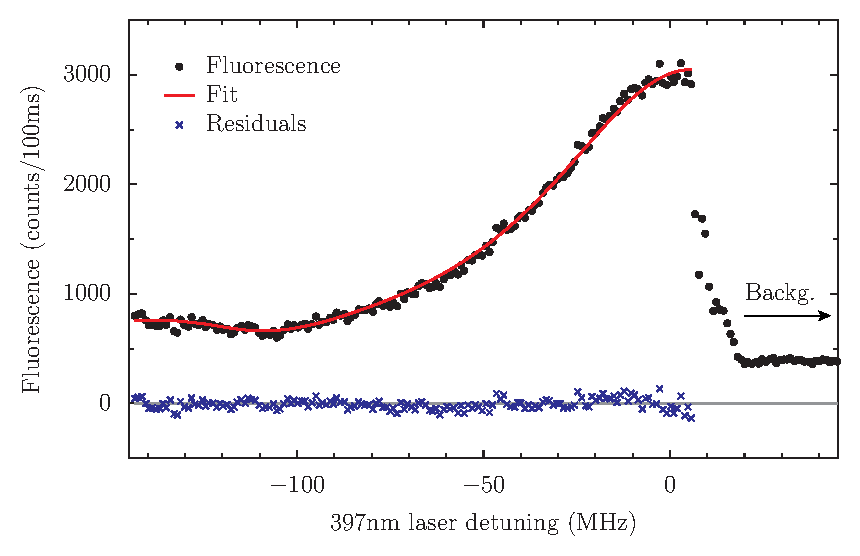
\includegraphics{chapter7/saturation/397satfit_v5}
\caption[Saturation scan fit example]{Example of fitted saturation profile. Laser parameters are $I_{397} = 6.39 I_{S,397}$, $I_{866} = 294.9 I_{S,866}$, $\Delta_{866} = -119.6\MHz$. Other fitting parameters are listed in Table~\ref{tab:satfitparams}. The measured power on the photodiode was 13\uW. The dropout on the blue side of the resonance is due to heating effects. The fluorescence  for 397\nm\, laser detunings between 20\MHz\, and 40\MHz\, are considered to be only the background, as subsequent scans show the ion was lost. The background level is estimated from a total of 300 points.}
\label{fig:satexamplefit}
\end{figure} 

\begin{figure}[h!t]
\centering
%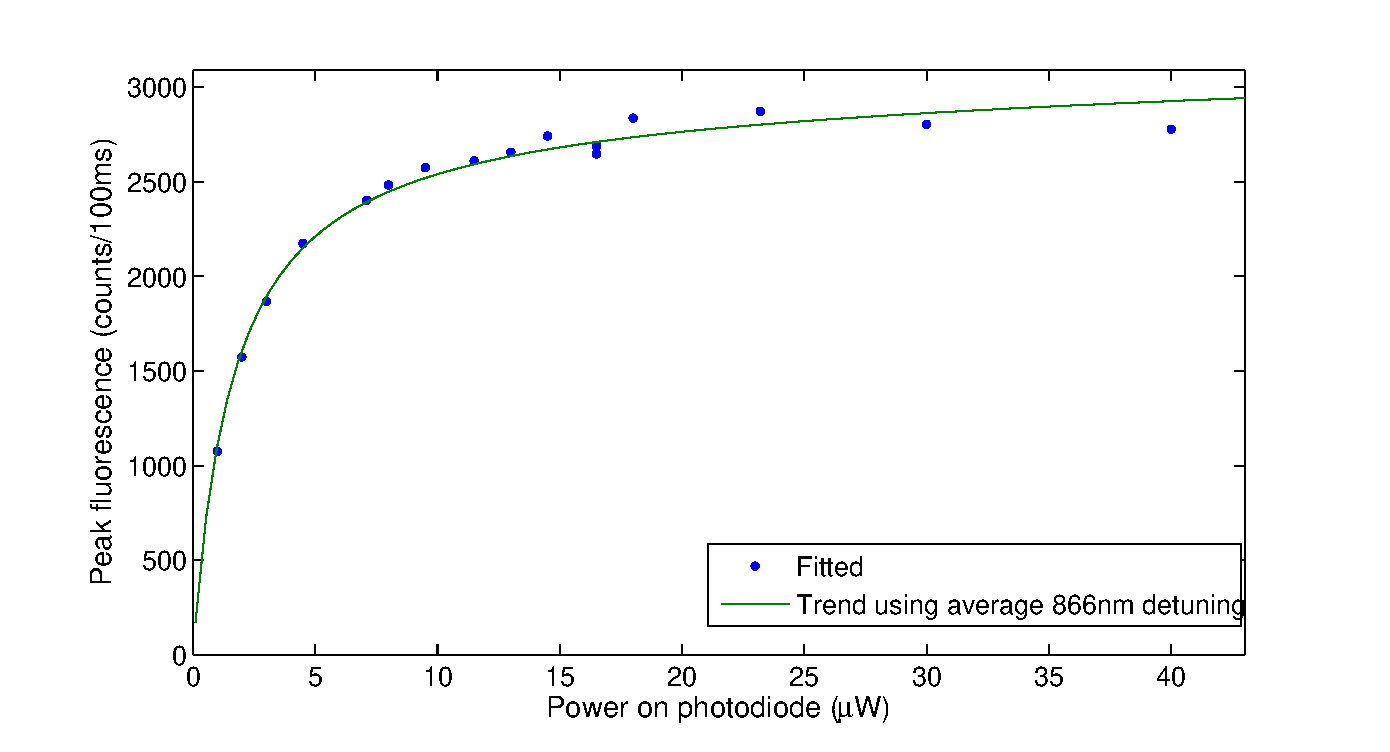
\includegraphics[width=12.5cm]{chapter7/saturation/397sat_v2}
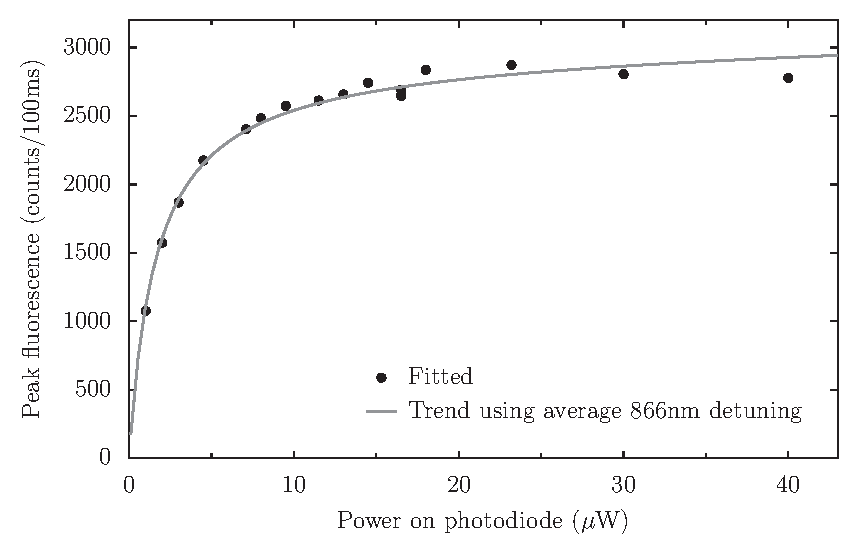
\includegraphics{chapter7/saturation/397sat_v3}
\caption[397\nm\, laser saturation curve]{Fitted peak fluorescence counts as a function of power on the photodiode. To show the general trend, the solid line is drawn using the mean of the fitted 866\nm\, laser detunings for all different 397\nm\, laser powers.}
\label{fig:397saturation}
\end{figure} 

\begin{figure}[h!t]
\centering
%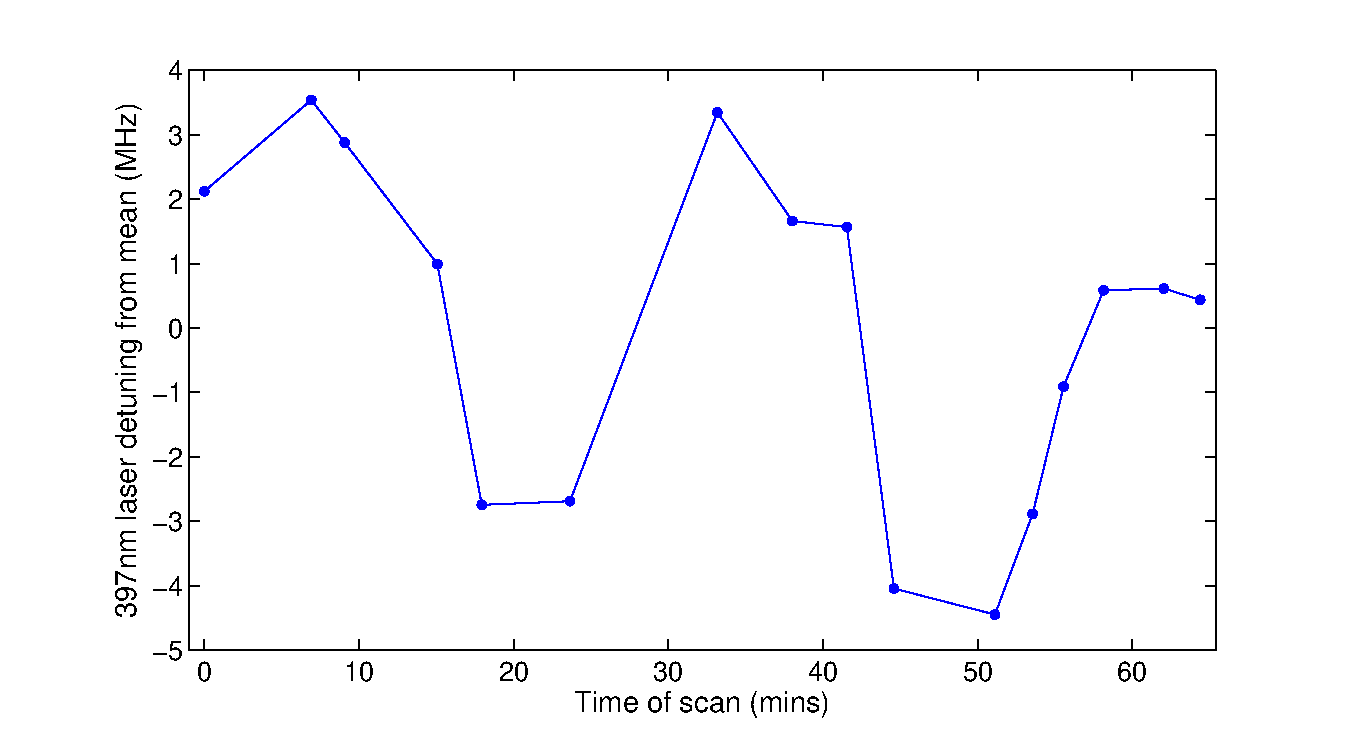
\includegraphics[width=12.5cm]{chapter7/saturation/397detuning_v2}
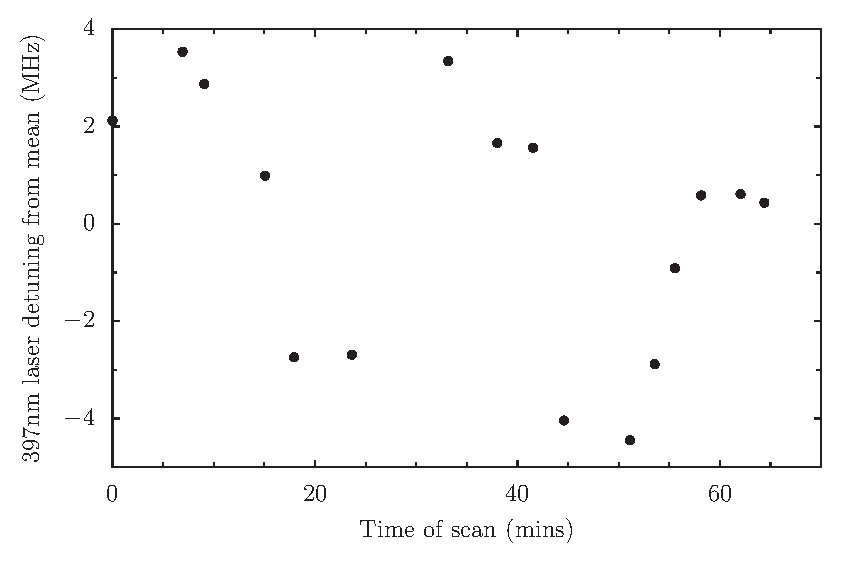
\includegraphics[width=12.5cm]{chapter7/saturation/397detuning_v3}
\caption[Change of 397\nm\, laser frequency versus time]{Change of the 397\nm\, laser frequency tuning as a function of time, shown as detuning from the mean value. The change in frequency is deduced from the fitted atomic resonance position. The change appears to be periodic, with a $\approx28\min$ period, similar to a cycle of the air-conditioning system.}
\label{fig:397resonancepos}
\end{figure} 


\section{Heating Rate}

The scope of what can be achieved with a given ion trap depends on the motional heating rate of trapped ions. For reliable large scale operation, low heating rates are desired, since high heating rates potentially limit ion lifetimes and length of quantum logic gate operations, as well as requiring more elaborate cooling and error correction schemes.

The relatively short ion lifetime in the absence of laser cooling in the Sandia trap suggested a large motional heating rate. To quantify this observation a method recently developed by the NIST Ion Trap Group was used \cite{Wesenberg2007}. The method is based on time-resolved measurement of ion fluorescence during Doppler cooling; it was chosen because it is capable of measuring high ion temperatures and required no additional equipment besides the two Doppler-cooling lasers and fast PMT already being used. 

An outline of the temperature measurement procedure is as follows. The Doppler-cooling is turned off for a certain amount of time (delay time, $\tau_d$), by turning off either of the two laser beams. When the Doppler-cooling is turned back on, the ion's fluorescence is recorded with fine time-resolution. The process is repeated a large number of times. The fluorescence as a function of time since the start of Doppler-cooling is fitted by a theoretical curve. In the simplest description, when the ion is assumed to have 1D motion and all laser parameters are known, the theoretical curve is described by a single parameter, the average temperature of the ion at the start of Doppler-cooling.

This method has been used by the NIST group to measure the motional heating rate of \mbox{$^{25}$Mg$^+$} ions in a microfabricated trap \cite{Epstein2007}. One significant difference in the case of \Ca{40} is that it has a $\Lambda$ level structure (we used the \soh-\poh-\dth\, levels, see Figure~\ref{fig:levels}), as opposed to the single cycling transition used in \mbox{$^{25}$Mg$^+$}. The ion experiences two different Doppler-shifts of the two lasers used for cooling, and requires fully numerical treatment, while the cycling transition has a good analytical description in the low laser saturation limit.

\subsection{Theoretical description}

The description of the ion's motion in 1D is as follows. The ion is assumed to be in the weak-binding regime in the $z$ direction, when the ion's motional frequency $\omega_z$ is much smaller than the excited state decay rate $\Gamma$. Thus the level populations are approximately in steady state, for any given value of the instantaneous effective detuning
\be
\Delta_{\mbox{eff}} = \Delta + \Delta_D
\ee
where $\Delta$ is the laser's detuning from the resonance, and $\Delta_D = - k_z v_z$, where $v_z$ and $k_z$ are the components of the velocity and the wave vector in the $z$ direction. 

The population $\rho_{22}(v_z)$ of the \poh\, excited state is then calculated by solving the Bloch equations, taking into account the effective detunings of the two Doppler-cooling lasers at different ion velocities (see Figure~\ref{fig:dbroadprofile}). 

Then the scattering rate is 
\be
\frac{\der N}{\der t} = \Gamma \rho_{22}(v_z)
\label{eq:dndt}
\ee
and the velocity-dependent force experienced by the ion is
\be
F_z(v_z) = m \frac{\der v_z}{\der t}= \hbar k_z \Gamma \rho_{22}(v_z).
\ee
The change in the ion's energy $E$ due to this velocity dependent force is averaged over one motional cycle:
\be
\frac{\der E}{\der t} = \langle v_z F_z (v_z) \rangle
\label{eq:dedt}
\ee
(see Figure~\ref{fig:dbroadprofile} and \ref{fig:dedt}). In the averaging the probability distribution of velocities is assumed to be that appropriate to harmonic motion:
\be
P(v_m,v) = \left\{
\begin{array}{cl}
\frac{1}{\pi}\frac{1}{\left(v_m^2 - v^2\right)^{1/2}} & \mbox{if } |v| < v_m\\ 
 & \\
0 & \mbox{otherwise }
\end{array}
\right.
\ee
where $v_{m}$ is the maximum velocity of the ion at the given motional energy.

Starting at a given ion motional energy $E$, equation~\ref{eq:dedt} is numerically integrated to calculate the cooling curve for the ion $E(t)$, and thus $v_m(t)$. Averaging Equation~\ref{eq:dndt} for one motional cycle, as a function of $v_m(t)$, one gets the fluorescence rate of the ion as a function of time (see Figure~\ref{fig:populationdop} and \ref{fig:cooling_fit}).

To calculate the predicted fluorescence from a large number of experimental repeats, we assume that the temperature after the heating delay is distributed according to the Maxwell-Boltzmann distribution, where the probability of having motional energy $E$ is
\be
P(E) = \frac{1}{\bar E} e^{-E/\bar E}
\label{eq:mbprob}
\ee
where $\bar E$ is the mean energy. The calculation of the fluorescence rate as a function of time is repeated for a number of motional energies, and averaged using the probability distribution of Equation~\ref{eq:mbprob}.

Figure~\ref{fig:cooling_fit} shows a fit of 1D motional theory to the recorded fluorescence, in the case of a delay time $\tau_d = 505\ms$ to allow the ion to heat up before the cooling lasers were switched on. The fitted temperature at the start of the cooling is $T = 31.3\pm2.0K$. In \cite{Epstein2007} the temperature derived from simple 1D motional model was compared to results of different temperature estimation (Raman sideband cooling), and found to be consistent. Both \cite{Epstein2007} and our experiments had similar geometrical arrangement: the laser beam that drives the fluorescence had its $k$ vector at 45\degree\, to the axial mode and one of the transverse modes, and close to perpendicular to the other transverse mode. The ion's motion could thus be assumed to be 2-dimensional only as the third mode is barely affected by the laser beam. It was modelled by 1D-cooling in both modes equally since the laser has the same $k$ in both directions due to its incidence angle.

When the radial motion is assumed to be unaffected by heating, or the heating rate is proportional to $\omega^{-1.4}$ (as has been found in other studies), the fitted temperature is similar to the 1D model. When the heating rate is assumed to be independent of $\omega$, the resulting fitted ion temperatures are reduced to about 40\% of that obtained from the 1D model. These results suggest that the 1D model describes the cooling process reasonably well, and the uncertainty of the heating rate measurement is more likely to be influenced by the changing environment and uncertainty in experimental control parameters.


\subsection{Effect of filtering the DC electrode lines}
\label{sec:filternoise}

Using the method described above, a comparison was made between the heating rate with unfiltered DC control voltages, and with a low-pass filter to reduce electrical noise on the electrodes. Figure~\ref{fig:dacnoise} shows the recorded noise spectrum for the DC lines when powered by the computer-connected DAC. The axial frequency of the trap is generally in the region of 300-800\kHz, so that the ion's axial motion is likely be excited by the noise on the DC line.

The heating rate was measured first without a filter (the situation for all the previous experiments), then the filter was installed and the measurement repeated (see Section~\ref{sec:dcelectrodecontrol}). Figure~\ref{fig:filter_heating} shows that the heating rate is significantly reduced by the filters from $206\pm80\K/\s$ to $60\pm9\K/\s$. An improvement in ion lifetime is also observed.

With the reduced noise on the DC electrodes, it was also possible to have even longer delay times, as it is shown on Figure~\ref{fig:long_heating_rate}. The longest delay time at which the experiments were repeatable was $\tau_d = 755\ms$. Times up to 1\s\, were observed occasionally, with loss a rate of a few per cent. 

The heating rate was fitted to be $49\pm8\K/\s$, which is in reasonable agreement with the previous experiment (experiments were conducted on different days). The mean occupation number is expressed from the temperature as
\be
\langle n \rangle = \frac{1}{e^{\hbar \omega / \kB T } - 1}
\ee
where $\omega$ is the trap frequency. For the axial motion of the ion with $\omega_{z} = 2\pi \times 800\kHz$ trap frequency, the measured heating rate corresponds to $\der\langle n \rangle/\der t\approx1.26\pm0.20\times10^{6}s^{-1}$. 

The electric field noise spectral density is calculated as
\be
S_E(\omega) \approx \frac{\der \langle n \rangle}{\der t}\frac{4m\hbar \omega}{e^2}
\ee
where $m$ is the ion's mass and $e$ is the elementary charge \cite{Turchette2000}. In the Sandia system, then
\be
S_E(\omega) \approx 6.9(\pm 1.1)\times 10^{-9} \V^2\m^{-2}\Hz^{-1}
\ee
which is higher than most other traps in the literature, but fits into the general trend (see Figure~\ref{fig:noise_spectra}). 

The heating rate we infer from our observations is high. When compared with results reported in the literature for other ion traps, it is at the upper end of the range for traps of the same physical dimensions. This means that in practice this trap, as it stands, is not a viable candidate for the implementation of quantum computing. There is a
chance that better filtering could reduce the electric field noise, but given that other groups reported severe problems with this sort of trap, it is more likely that the problems are mainly intrinsic to the trap itself. The evidence from the wider study of small traps in general is that they experience electric field noise due to some as yet unclear unstable behaviour at the electrode surfaces, such as fluctuating  patch potentials. There is some evidence (partly anecdotal) that the choice of materials and the smoothness of the electrode surfaces is important. Rather than test the Sandia trap further (for example by attempting sideband cooling) it was decided to move on to other traps, and recommend that the next stage for this design should include a more complete gold coating, and a better surface smoothness. Both are especially important for the surfaces nearest to the ion or ions.


\begin{figure}[h!t]
\centering
%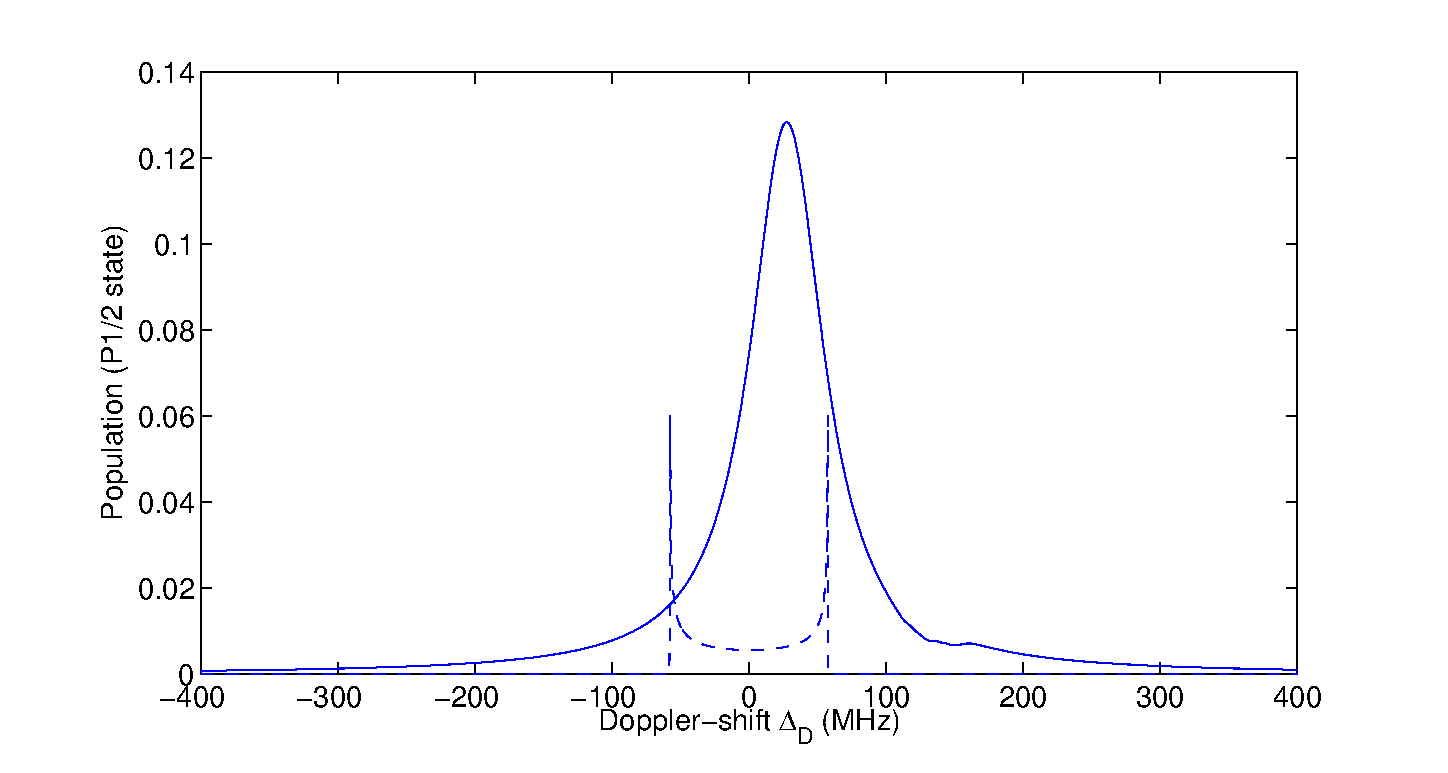
\includegraphics[width=14.5cm]{chapter7/heating/sample_dopplerpop}
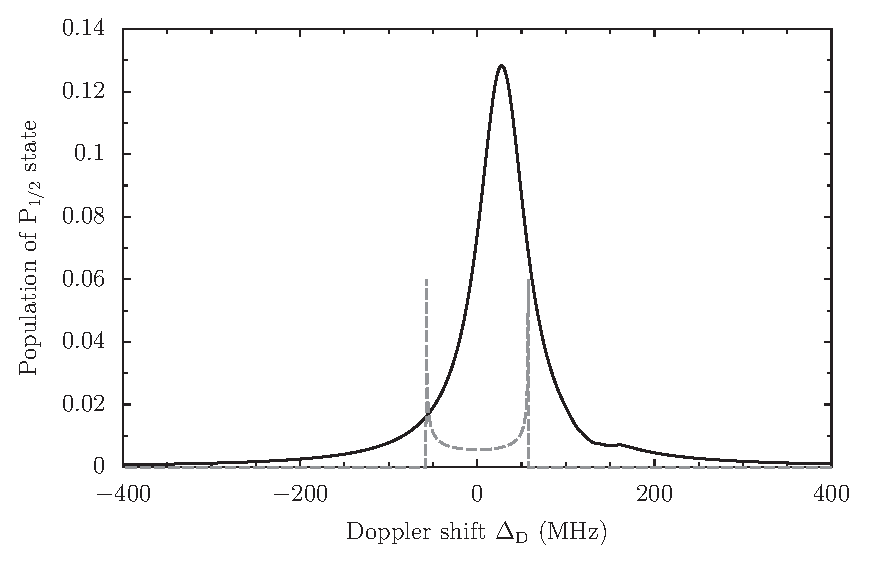
\includegraphics{chapter7/heating/sample_dopplerpop_v2}
\caption[Doppler-broadened fluorescence profile]{Population of the \poh\, level as function of Doppler-shift $\Delta_D=-k_zv_z$. The probability distribution of the Doppler-shift in case of maximal cooling rate is shown by the dashed line. Experimental control parameters (laser intensity, detuning, magnetic field) are as in Figure~\ref{fig:cooling_fit}.}
\label{fig:dbroadprofile}
\end{figure} 

\begin{figure}[h!t]
\centering
%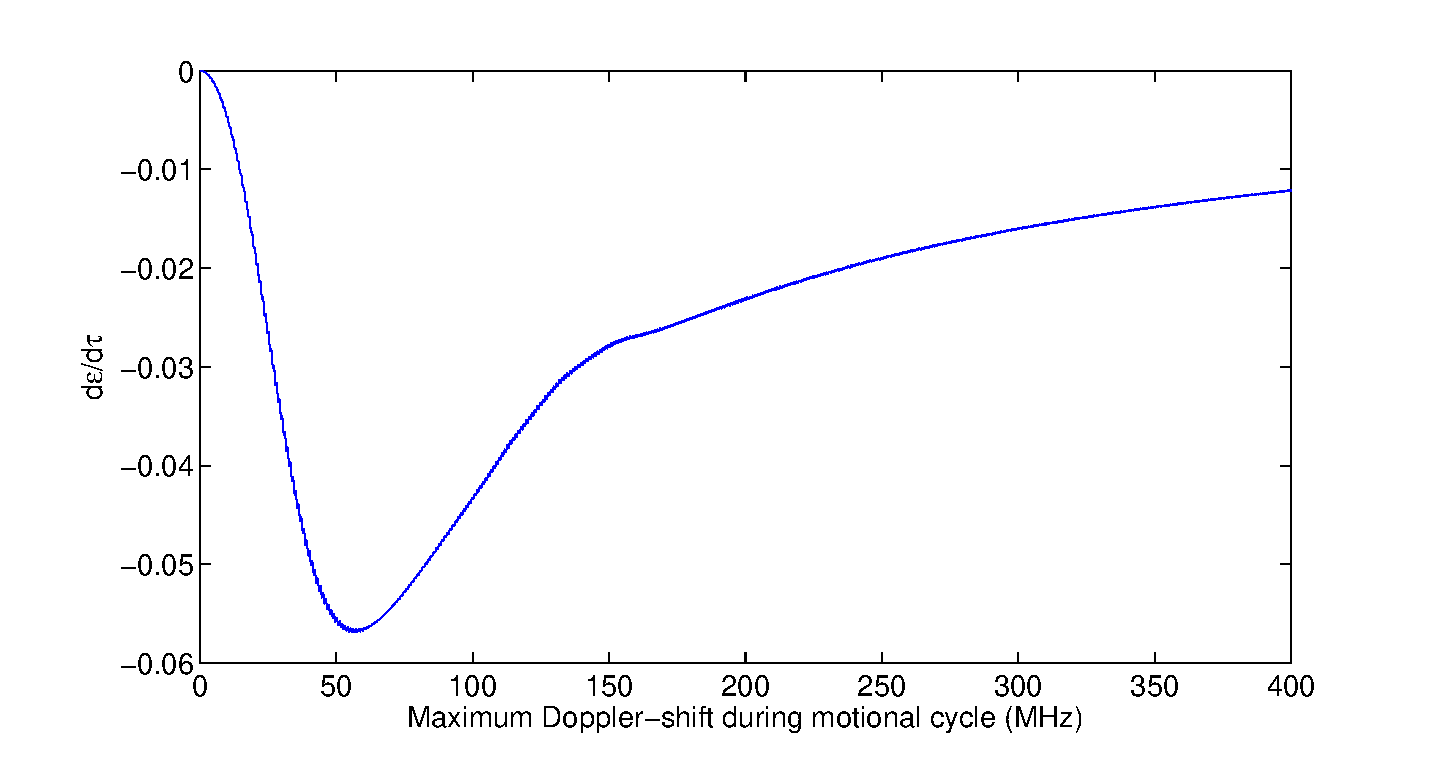
\includegraphics[width=14cm]{chapter7/heating/sample_dedt}
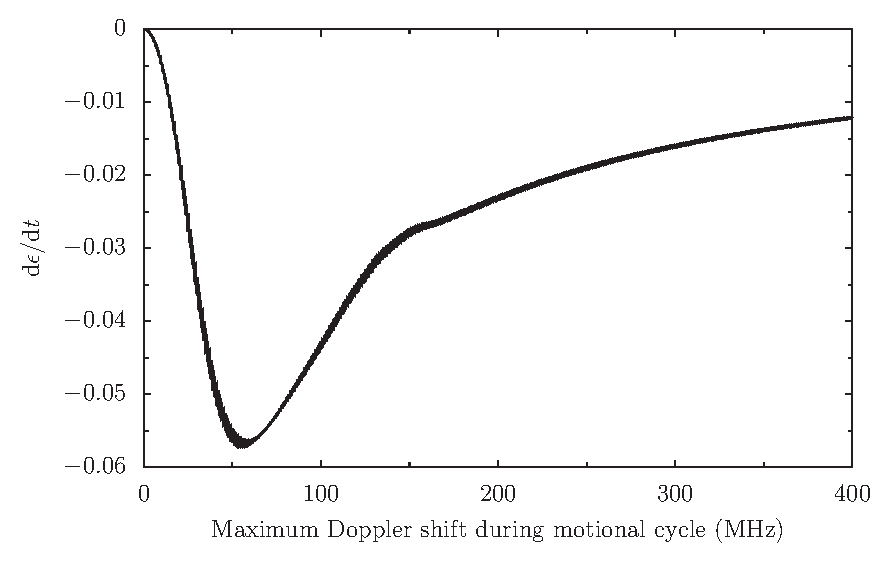
\includegraphics{chapter7/heating/sample_dedt_v2}
\caption[Cooling rate versus maximum ion velocity]{The rate of change in ion energy as function of the maximum Doppler shift of the ion's motion. The energy is scaled by $E_0 = \hbar \Gamma$, and the time by $t_0 = \Gamma^{-1}$, where $\Gamma = 2\pi \times 22.4\MHz$ is the excited state decay rate. Calculated from curves shown in Figure~\ref{fig:dbroadprofile}.}
\label{fig:dedt}
\end{figure} 

\begin{figure}[h!t]
\centering
%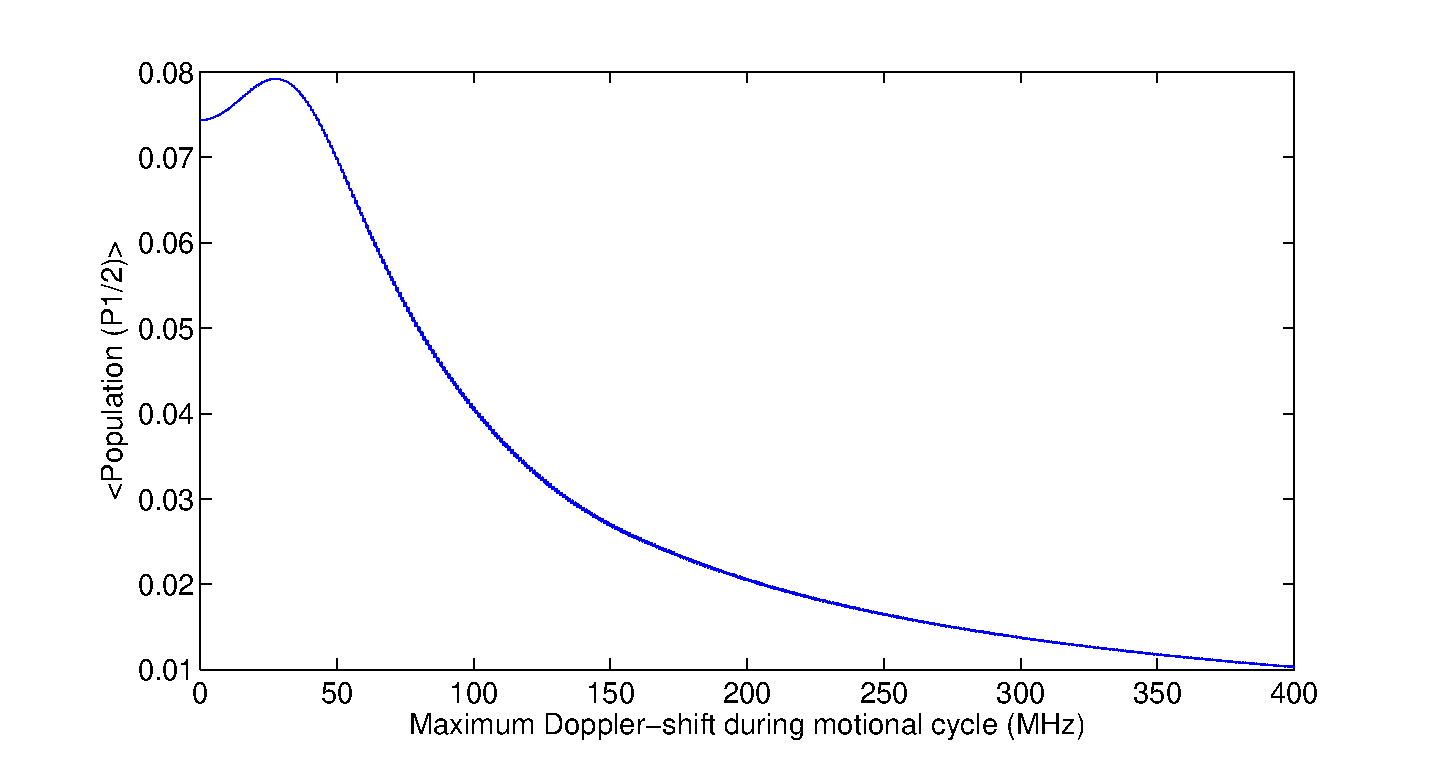
\includegraphics[width=14cm]{chapter7/heating/sample_population}
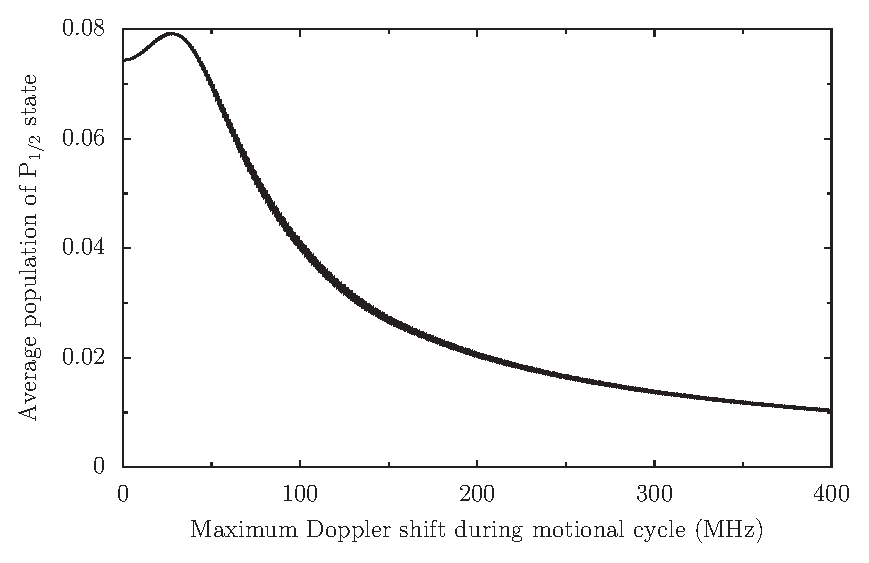
\includegraphics{chapter7/heating/sample_population_v2}
\caption[Population of excited level versus maximum ion velocity]{Average population of the \poh\, level as a function of the maximum Doppler shift of the ion's motion. The scattering rate is $\Gamma$ times the population of the \poh\, level. Calculated from curves shown in Figure~\ref{fig:dbroadprofile}.}
\label{fig:populationdop}
\end{figure} 

\begin{figure}[h!t]
\centering
%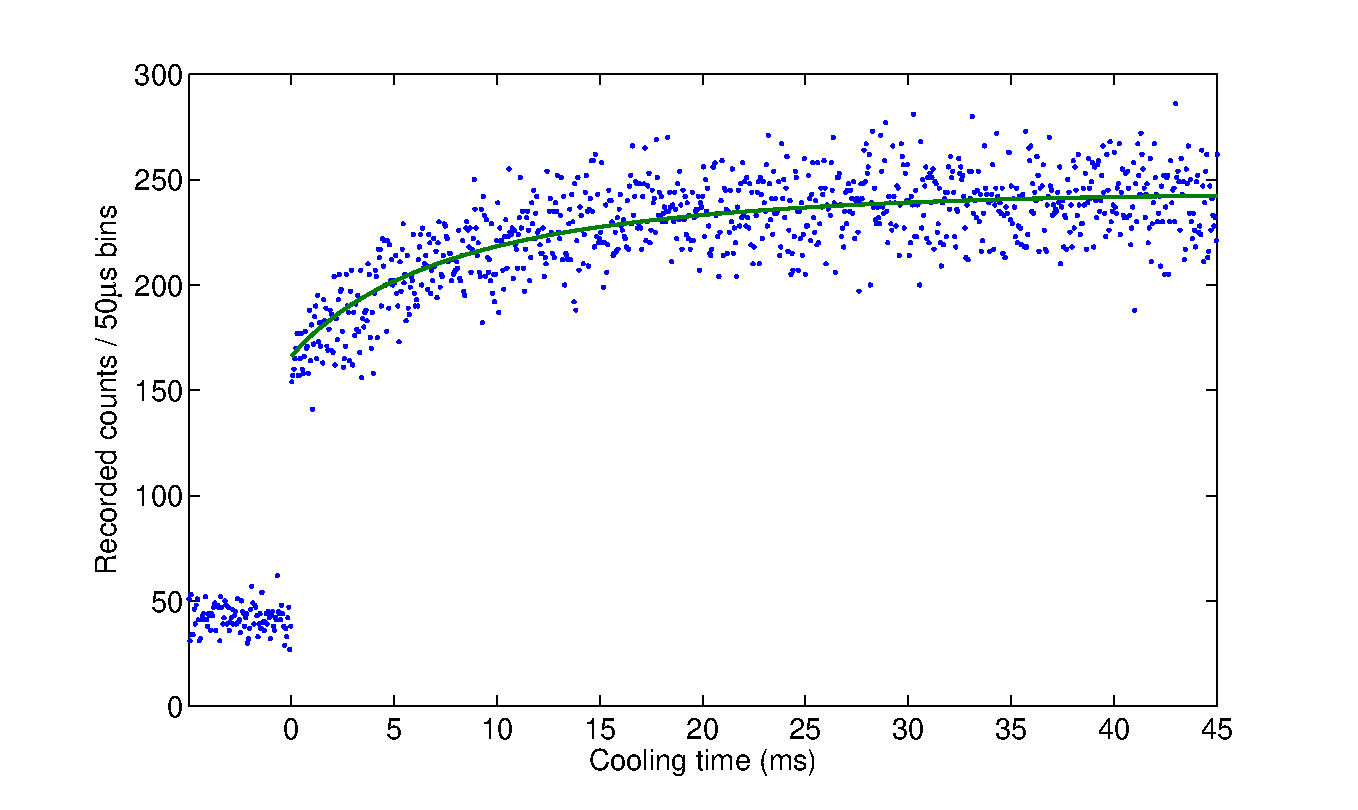
\includegraphics[width=14.5cm]{chapter7/heating/cooling_fit_v2}
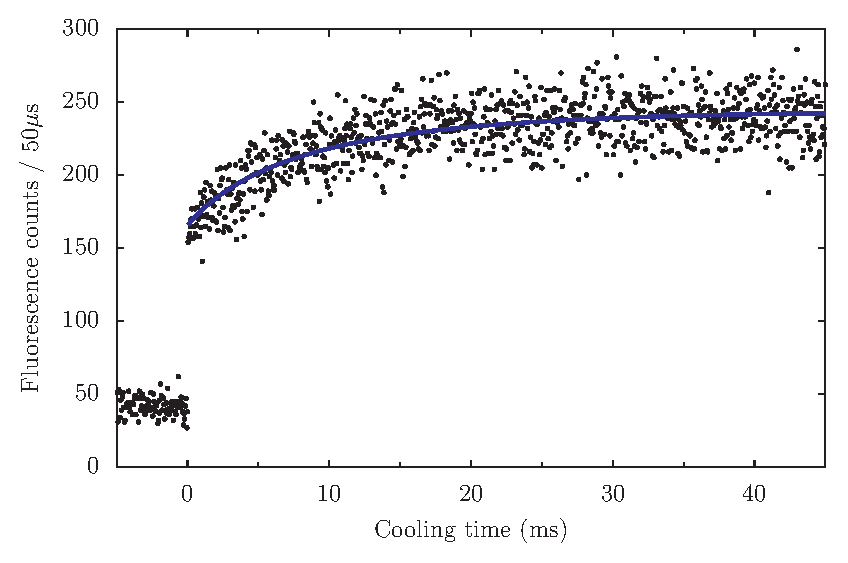
\includegraphics{chapter7/heating/cooling_fit_v3}
\caption[Example fit of fluorescence during Doppler-cooling]{Time-resolved fluorescence during Doppler cooling. Cooling starts at $t=0$. Delay time 505\ms, 301 repetitions, fluorescence is recorded in 50\us\, bins. The signal at $-5\ms~\le~t~\le~0$, before the cooling is turned on, is used to fit the background.  The fitted temperature is $T = 31.3\pm2.0\K$. Experimental parameters are $I_{397}~=~3.2I_{S,397}$, $I_{866}~=~39I_{S,866}$, $\Delta_{397}~=~-34.2\MHz$, $\Delta_{866}~=~39.0\MHz$, $B~=~3.6\G$, $\phi_{397}~=~\pi/4$, $\phi_{866}~=~\pi/2$.}
\label{fig:cooling_fit}
\end{figure} 


\begin{figure}[h!t]
\centering
%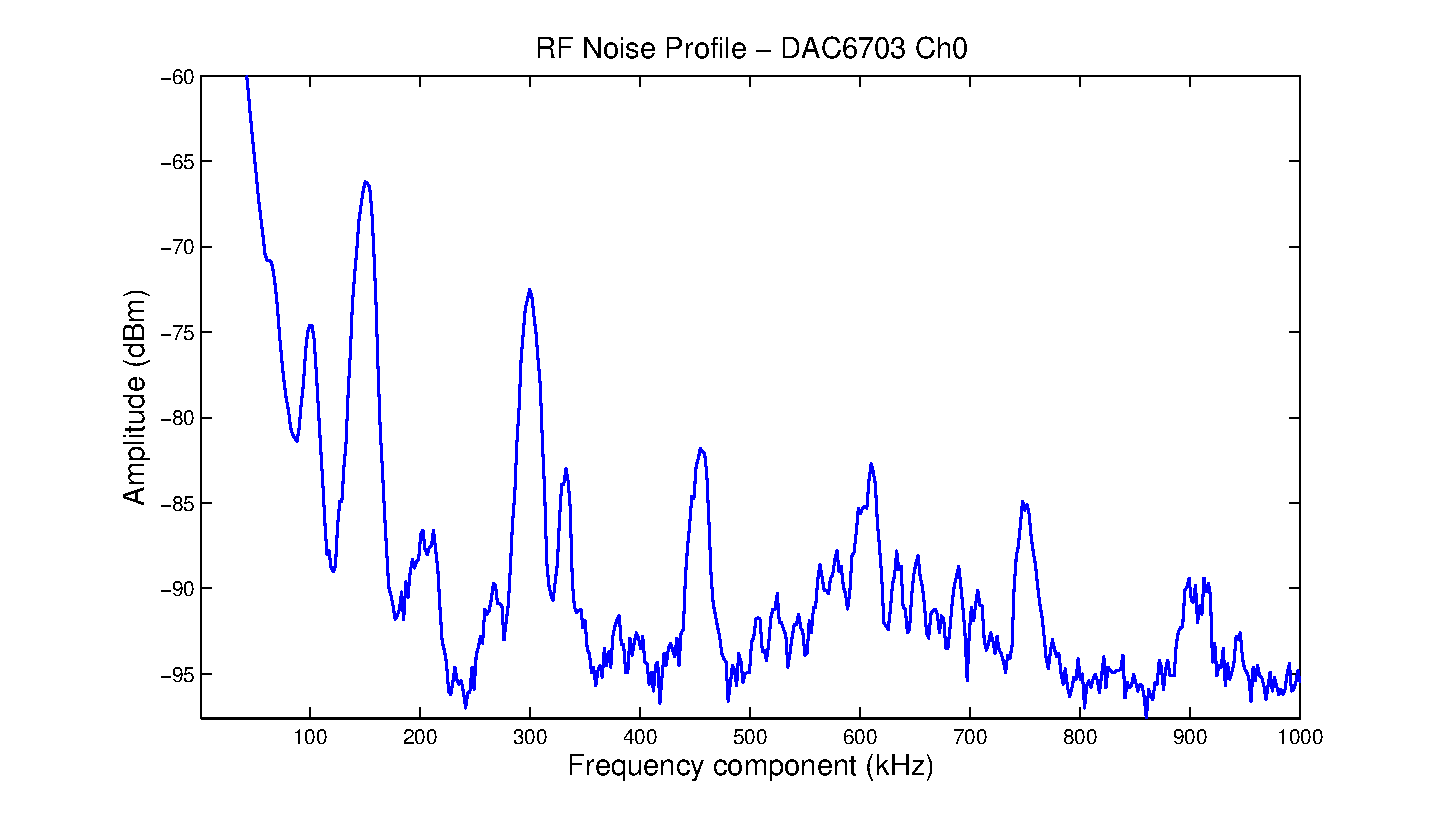
\includegraphics[width=14.5cm]{chapter7/noise/dacnoise}
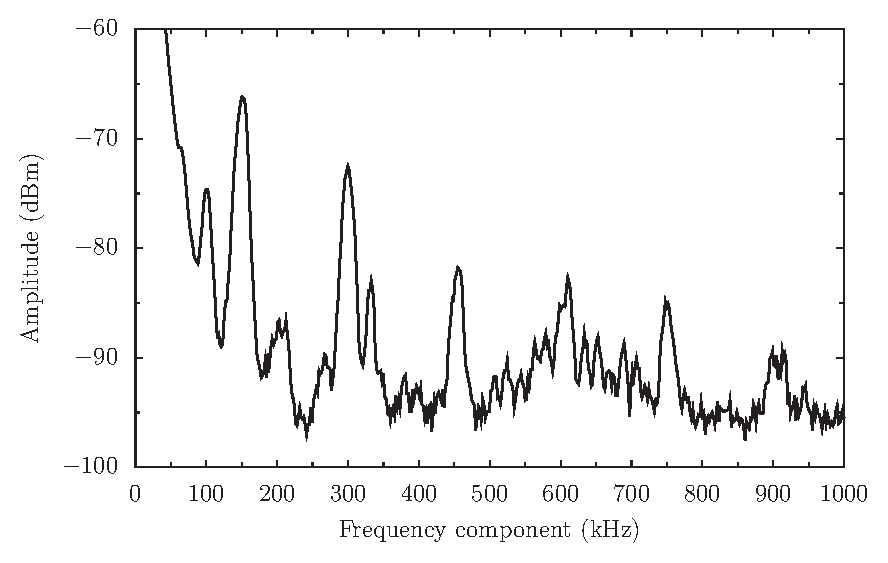
\includegraphics{chapter7/noise/dacnoise_v2}
\caption[DAC noise Fourier spectrum]{DAC noise Fourier spectrum recorded with a Tektronix TDS2024 oscilloscope. High harmonics of 100\kHz\, and 150\kHz\, are visible. The usual trap operation is in the 300-900\kHz\, axial frequency range.}
\label{fig:dacnoise}
\end{figure} 

\begin{figure}[h!t]
\centering
%\includegraphics[width=14.5cm]{chapter7/heating/filterheating_v3}
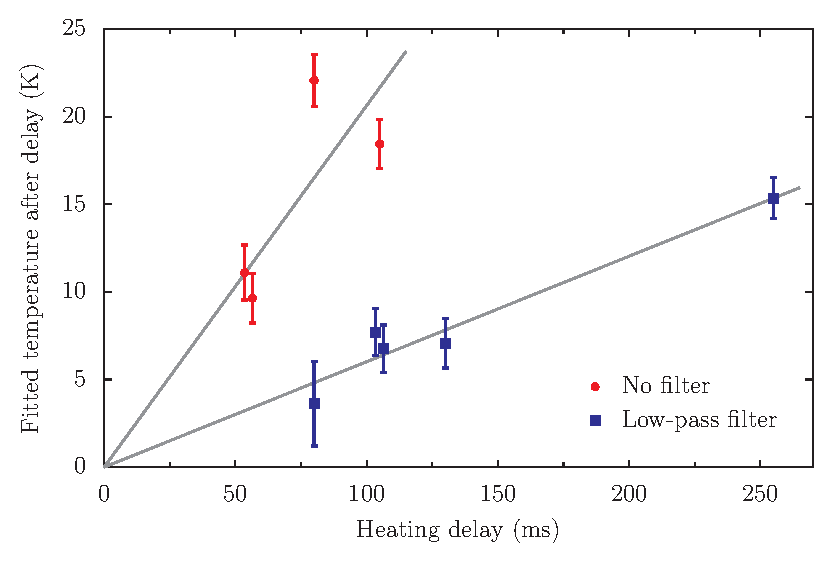
\includegraphics{chapter7/heating/filterheating_v4}
\caption[Ion's motional heating rate with/without DC filters]{Ion temperature after heating up as a function of heating delay, with and without low-pass filters installed on the DC voltage lines. The heating rate without the low-pass filters is $206\pm80\K/\s$, while with filters it is $60\pm9\K/\s$.}
\label{fig:filter_heating}
\end{figure} 

\begin{figure}[h!t]
\centering
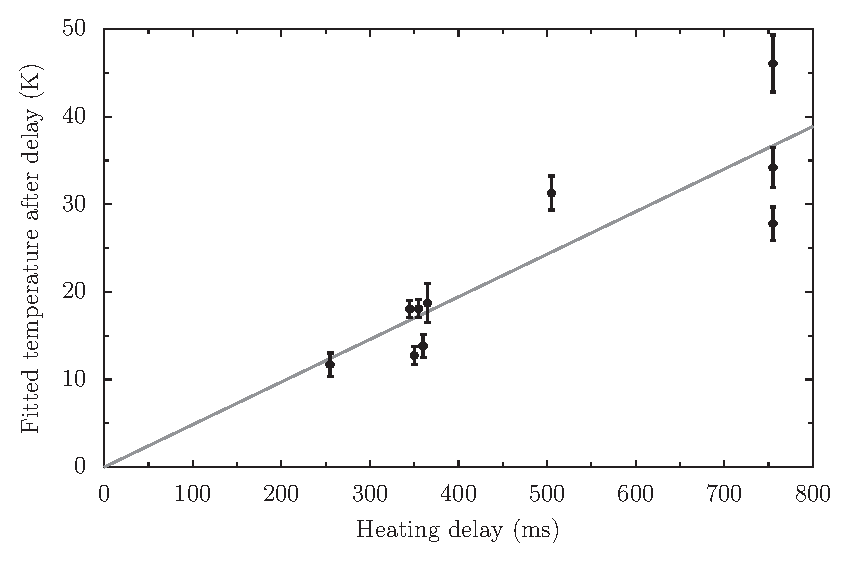
\includegraphics{chapter7/heating/long_heating_rate_v3}
\caption[Motional heating rate measurement with long delay times]{Heating rate measurement at long delay times, with DC line low-pass filters. All experiments were done with filters on the DC lines, and the best possible micromotion compensation. Delay times are $\tau_d =  \{255,355,505,755\}\ms$. The multiple measurements at 355\ms\, delay time would overlap too much on this plot, so they have been spread out slightly along the x-axis for clearer presentation. The heating rate is fitted as $49\pm8\K/\s$, which is similar to the heating rate shown in Figure~\ref{fig:filter_heating} (with filters).}
\label{fig:long_heating_rate}
\end{figure} 

\begin{figure}[h!t]
\centering
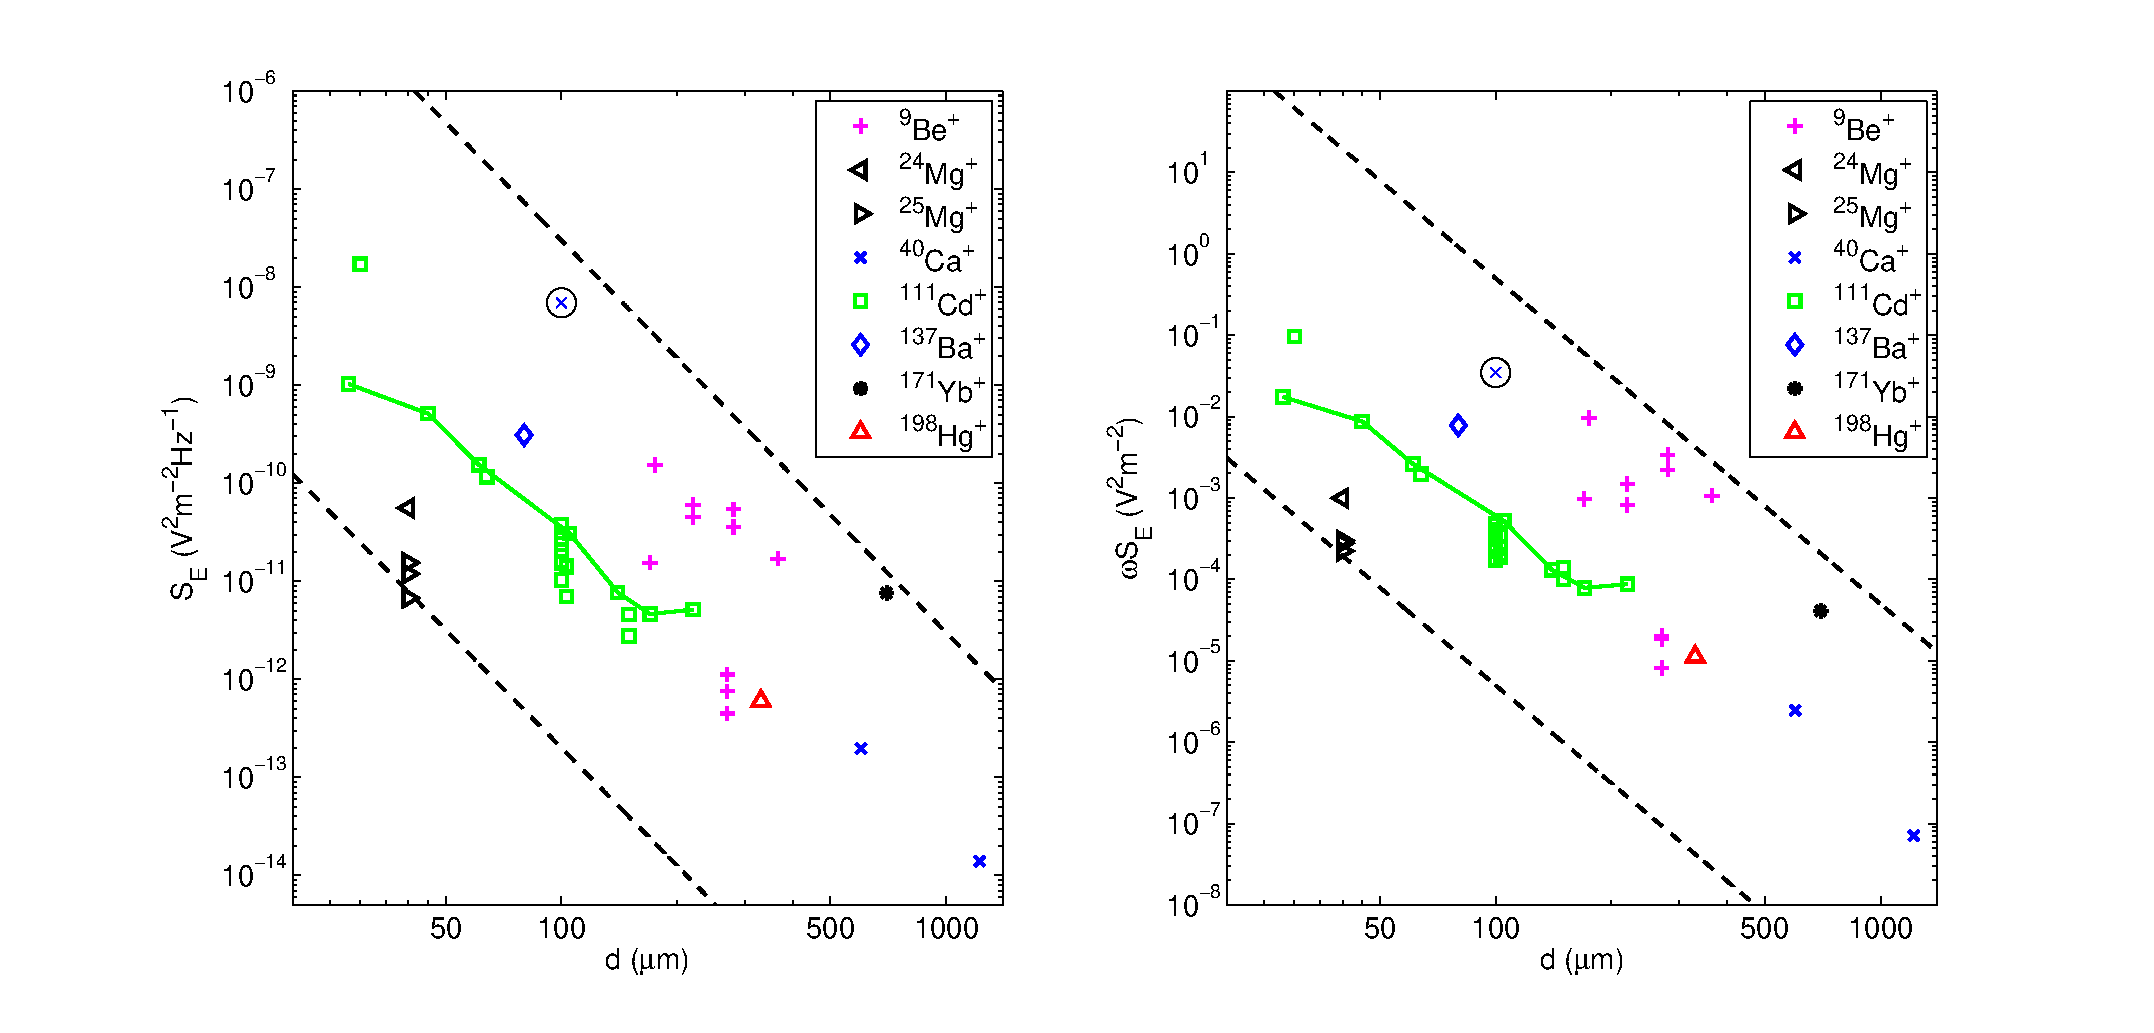
\includegraphics[width=15.5cm]{chapter7/heating/noise_spectra_v3}
\caption[Electric field noise spectral density]{Electric field noise spectral density $S_E(\omega)$ (left) and $\omega S_E(\omega)$ (right) for a number of different traps and ion species in the literature. The results of the present work is indicated by circles. References for the other data points: \ion{Be}{9}~\cite{Rowe2002,Monroe1995,Turchette2000} , \ion{Mg}{24}~\cite{Seidelin2006}, \ion{Mg}{25}~\cite{Epstein2007}, \ion{Ca}{40}~\cite{Roos1999,Home2006b}, \ion{Cd}{111}~\cite{Deslauriers2004,Stick2006,Deslauriers2006}, \ion{Ba}{137}~\cite{DeVoe2002}, \ion{Yb}{171}~\cite{Tamm2000}, \ion{Hg}{198}~\cite{Diedrich1989}. The data for the same trap is connected by a line. The dashed lines are paralled to $d^{-4}$. \cversion}
\label{fig:noise_spectra}
\end{figure} 



\section{Ion shuttling}
\label{sec:ionshuttle}
As mentioned in the Introduction, to scale up existing ion trap designs the problem of storage and manipulation of a large number of ions has to be addressed. Many current proposals of designs include different trap regions optimized for storing ions and for ion-ion interaction. The ions thus have to be moved between such regions with high speed and accuracy, while keeping the information stored in the ion's quantum state intact.

Ion shuttling has been demonstrated in other trap designs previously \cite{Huber2008}. The Sandia trap offered us an opportunity to get some initial experience of the issues involved. The shuttling of a single ion was studied in two experiments. 

In the first instance voltages on most electrodes were kept constant, and only the voltage of one pair of the outermost electrodes was changed (pair \#1 or \#7, see Figure~\ref{fig:sandiatrap}). By changing the voltage on these electrodes, the trapping potential's minimum was displaced from the geometrical trap centre. Because of symmetry, the displacement was along the trapping axis. The CCD camera had a field of vision with a length of approximately 120\um, limited by a pinhole in the imaging system. The 397\nm\, beam was elongated in the horizontal direction with a tilted focusing lens before the trap (see Section~\ref{subsec:dopplertrapsetup}) and the 866\nm\, beam had a large spot-size and high power. Thus the lasers stayed in interaction with the ion all the way through the field of view of the CCD camera, and the photon scattering could be observed.

The voltage on the electrode pairs of \#1 and \#7 was changed in steps, and a picture of the ion was taken. The length scale was calibrated by taking a picture of one of the centre electrodes with known width of 100\um. Figure~\ref{fig:stepmove} shows the ion's position as a function of the difference between the voltages on electrode pairs \#1 and \#7. The dataset contains position information from two ions, as the trap had to be reloaded once during the experiment. 
%The position of the ion is compared to simulation.


The second experiment was to demonstrate shuttling to large distances. The furthest trapping region from the trap centre is in front of the DC electrode pairs \#2 or \#6, since the outermost electrodes have to produce barrier fields, stopping the ion from leaving the trap along the trap axis. Thus the furthest available shuttle distance is $\pm360\um$ from the trap centre. Shuttling to such a distance requires changing the voltage on more than one electrode pair. In practice changing 4 out of the 7 DC voltages is sufficient. Depending on the required direction of movement the electrode pairs \#1 to \#4, or \#4 to \#7 have to be changed. Figure~\ref{fig:shuttlevolts} shows the applied voltage as a function of ion distance from the trap centre. 

In the experiment we shuttled the ion at a constant speed along the axis: the distance travelled along the trap axis was thus linear in time. This is a very crude initial approach, since significant ion heating is expected due to the ``kicking-and-stopping'' nature of the control. A smooth acceleration and deceleration would be desirable in practice, to minimize heating (see Section~\ref{sec:preciseshuttle}). However there are several factors which suggest that even the crude approach is acceptable in this case. The Sandia trap has such a high heating rate that the additional heating from the ion movement is probably not significant. To experimentally realize the waveforms whose theory was presented in Section~\ref{sec:preciseshuttle}, one needs much better timing resolution that was available to us at the time. Finally, the timescale of the shuttling experiment was in the order of milliseconds, which is close to adiabatic considering the ion motion timescale set by the trap frequency of 600-900\kHz.

The speed of the shuttling was limited by two factors. First, the DAC available at the time of the experiment (PCI-DAC6703) had a maximum 1111\Hz\, update rate (0.9\ms/update). Second, the RC filters on the DC voltage lines have time constants of $\tau = 0.18\us$. According to computer calculations to assess the effect of the  RC filters, the voltage waveforms were not significantly changed at the maximum update rate of the DAC card. However, if a faster DAC were used, the RC filters would have to be changed to have a higher cut-off frequency. This would lead to a higher level of electric noise on the DC electrodes, thus giving a higher heating rate and shorter ion lifetime. The amount of extra heating one can afford to trade for higher shuttling speeds needs further investigation.

In the experiment, the ion was moved to the largest distance allowed in the shortest possible time. Experiments indicated that the required waveforms can be approximated in 10 steps without losing the ion during the shuttle (see Figure~\ref{fig:rtscopewaveform}). Less than a 10 step voltage change lost too much detail of the waveforms to provide a reliable shuttle. The 10 step waveform together with a set minimal update time of 1\ms\, provides a 10\ms\, shuttle time away and a 10\ms\, shuttle back to the trap centre. In the experiment a delay was applied before shuttling back to the starting position. For reliable timing, a real-time operating system was used (GNU/Linux 2.6.23\footnote{GNU/Linux Kernel, \url{http://www.kernel.org/}} , Xenomai\footnote{Xenomai Real-Time Framework, \url{http://www.xenomai.org/}} and Comedi\footnote{Linux Control and  Measurement Device Interface, \url{http://www.comedi.org/}}) which was superior to the DAC's own supplied control software under the Windows operating system. The reliability of timing is demonstrated in Figure~\ref{fig:rtscopewaveform}, where 20 repeats of the voltage waveform are recorded and show good repeatability. The remaining variability of the signal is partly due to the control electronics of the DAC: the order in which the output channels are updated seems to vary in every update round.

Figure~\ref{fig:longshuttle} shows a recorded fluorescence signal during shuttling of an ion when a 120\ms\, delay time was applied  between the outward and inward movement. With this delay time the ion was reliably shuttled more than 500 times. However, at larger delay times the ion was lost in a small number repeats.  The half a second delay between repeats is due to software limitations, as the hardware was reprogrammed before every shuttle.

According to the results in the previous section, the amount of time the ion stayed reliably in the trap after loss of cooling was in the order of 500-750\ms. The fact that the observed maximum delay to reliably shuttle an ion (120\ms) is shorter suggests that either the shuttle contributed to the heating of the ion or that the trapping at the end points is inherently less stable.

The ion shuttling described was paving the way for experiments with multiple ions, when ions are stored in different trapping regions. Based on the results of the ion shuttling, with Doppler-cooling beams at the different trapping regions in addition to the trap centre, it would be possible to keep ions for a significant amount of time while moving them. One additional aspect of the multi-ion experiment is the separating and joining of ion pairs in a trapping region. It is not clear whether the Sandia trap is capable of doing this; certainly, to be able to test any ion-pair manipulation method (such as the precise shuttling sequence in Section~\ref{sec:preciseshuttle}), the ion pair lifetime in the Sandia trap would need to be improved (see Section~\ref{sec:multiions}).

\begin{figure}[h!t]
\centering
%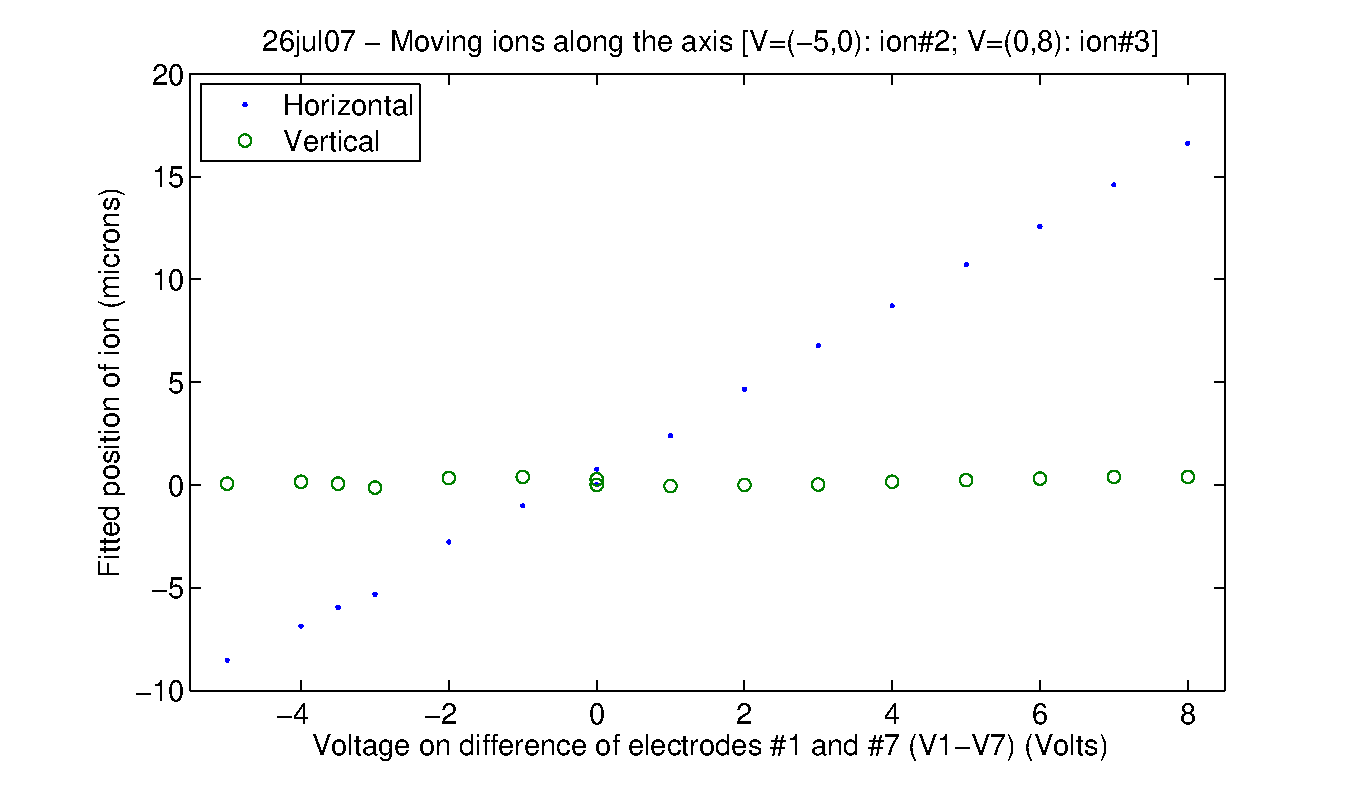
\includegraphics[width=14.5cm]{chapter7/ionmove/ionmove}
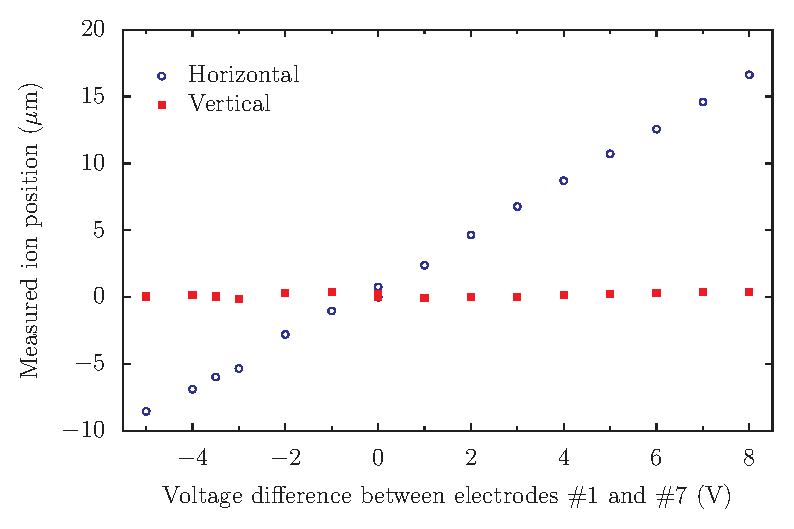
\includegraphics[width=14.5cm]{chapter7/ionmove/ionmove_v1}
\caption[Moving ion step by step with outermost electrode pairs]{Moving the ion step by step with the outermost electrode pairs. The ion's position is plotted versus voltage difference between the \#1 and \#7 electrode pairs. The position is deduced by CCD pictures and known scaling factor for the images.}
\label{fig:stepmove}
\end{figure} 


\begin{figure}[h!t]
\centering
%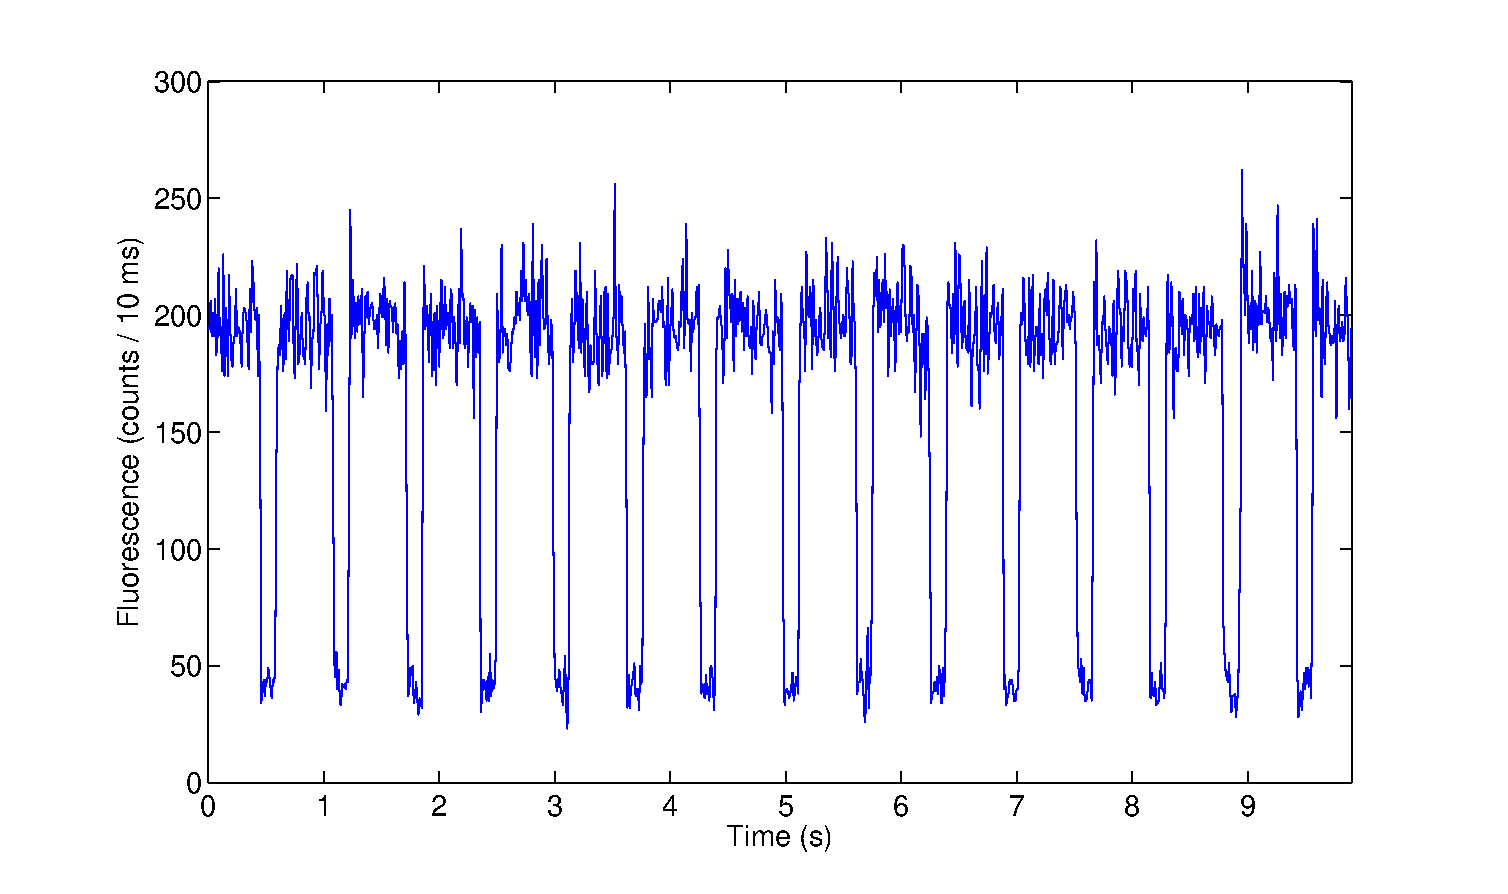
\includegraphics[width=14.5cm]{chapter7/shuttle/longshuttle}
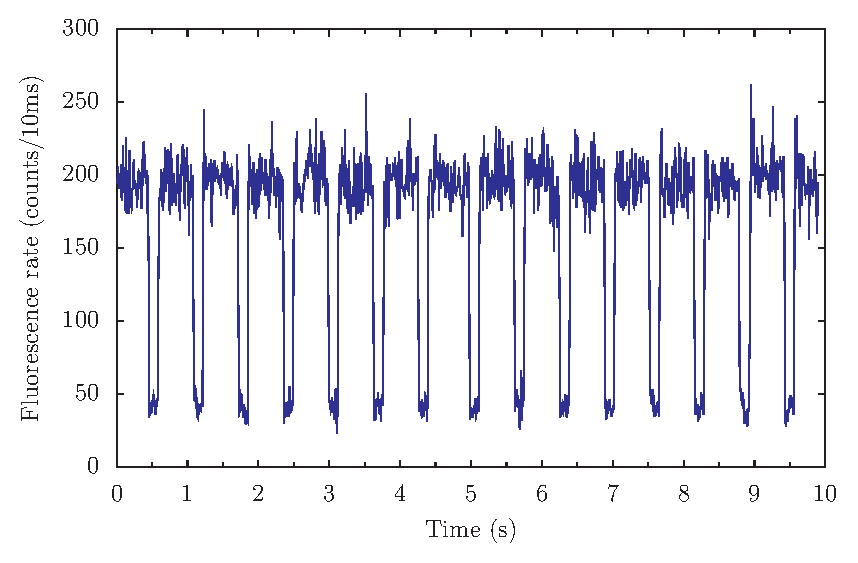
\includegraphics{chapter7/shuttle/longshuttle_v1}
\caption[Fluorescence during ion shuttle]{Fluorescence signal during ion shuttle. The outward and inward movement is 10\ms\, each, while a delay of 120\ms\, is applied between them. The shuttle repetition was limited to 1 every 700\ms\, due to the calculation overhead between shuttles.}
\label{fig:longshuttle}
\end{figure} 

\begin{figure}[h!t]
\centering
%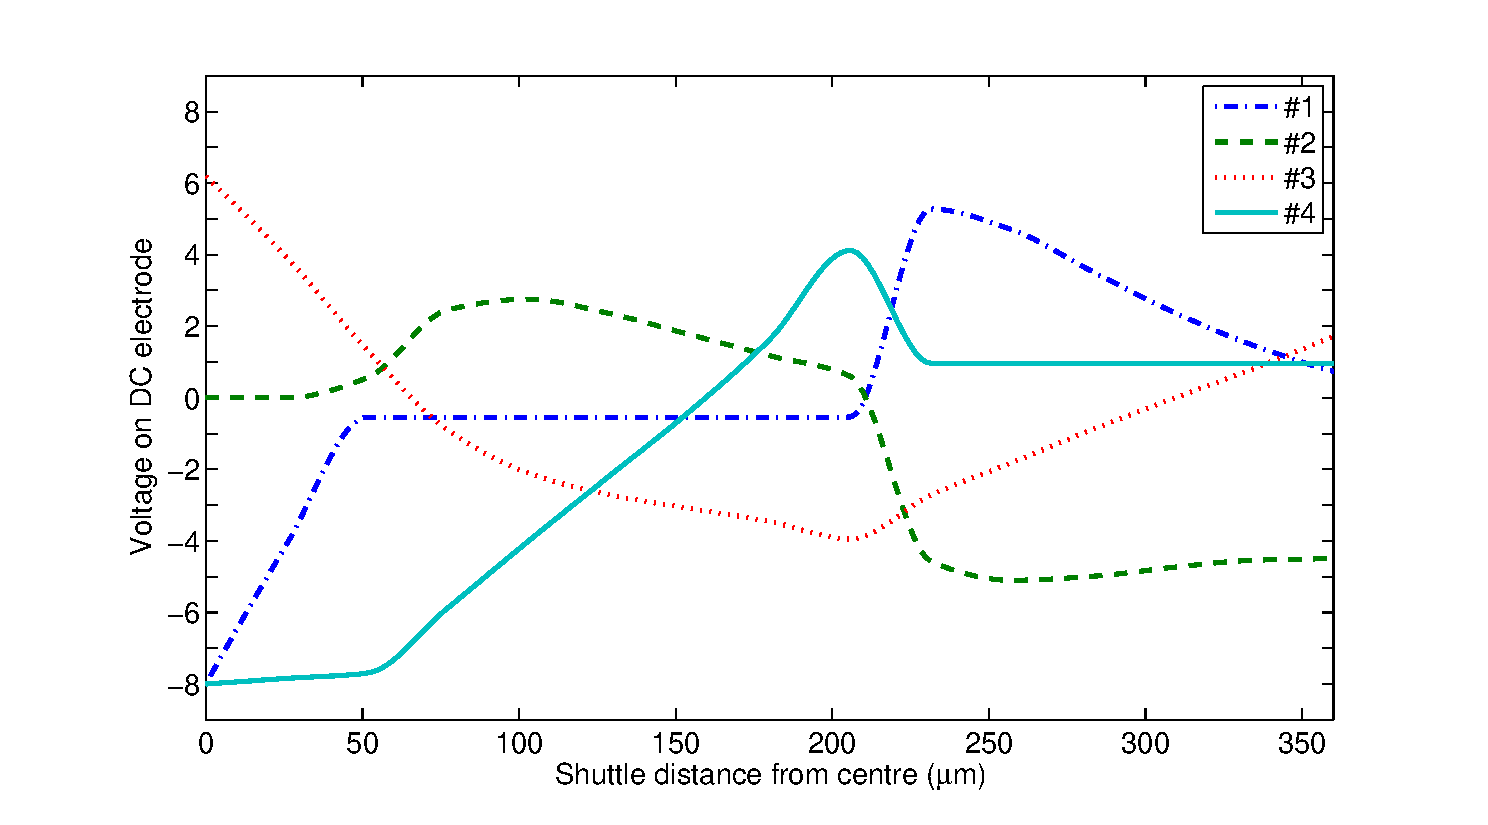
\includegraphics[width=14.5cm]{chapter7/waveform/rtusual/shuttlevoltage}
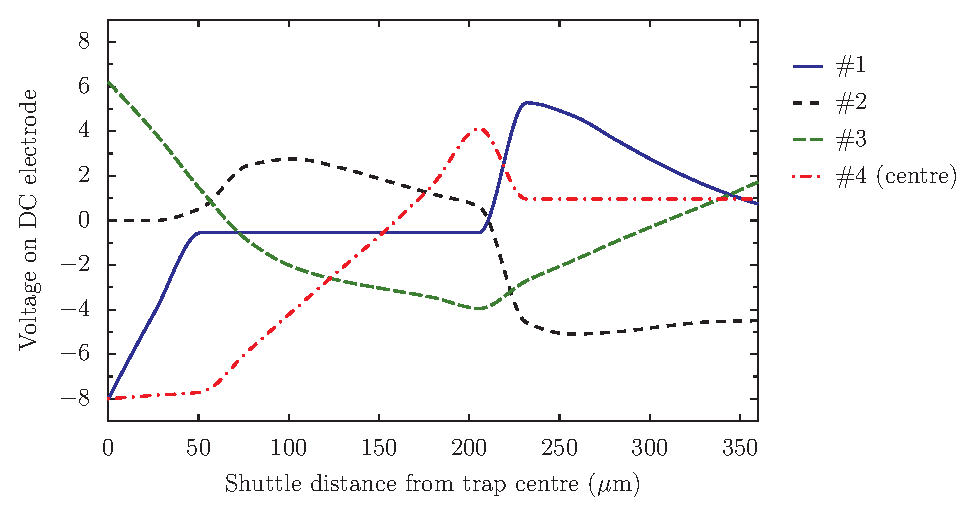
\includegraphics[width=14.5cm]{chapter7/waveform/rtusual/shuttlewaveform_v1}
\caption[DC electrode voltages for shuttle]{Voltages on DC electrodes as a function of ion's distance from trap centre. Only 4 of 7 possible voltages are plotted, as the other 3 voltages are kept constant during the shuttle. The electrodes used to shuttle ion to the left (right) are \#1,2,3,4  (\#7,6,5,4). }
\label{fig:shuttlevolts}
\end{figure} 




\begin{figure}[h!t]
\centering
%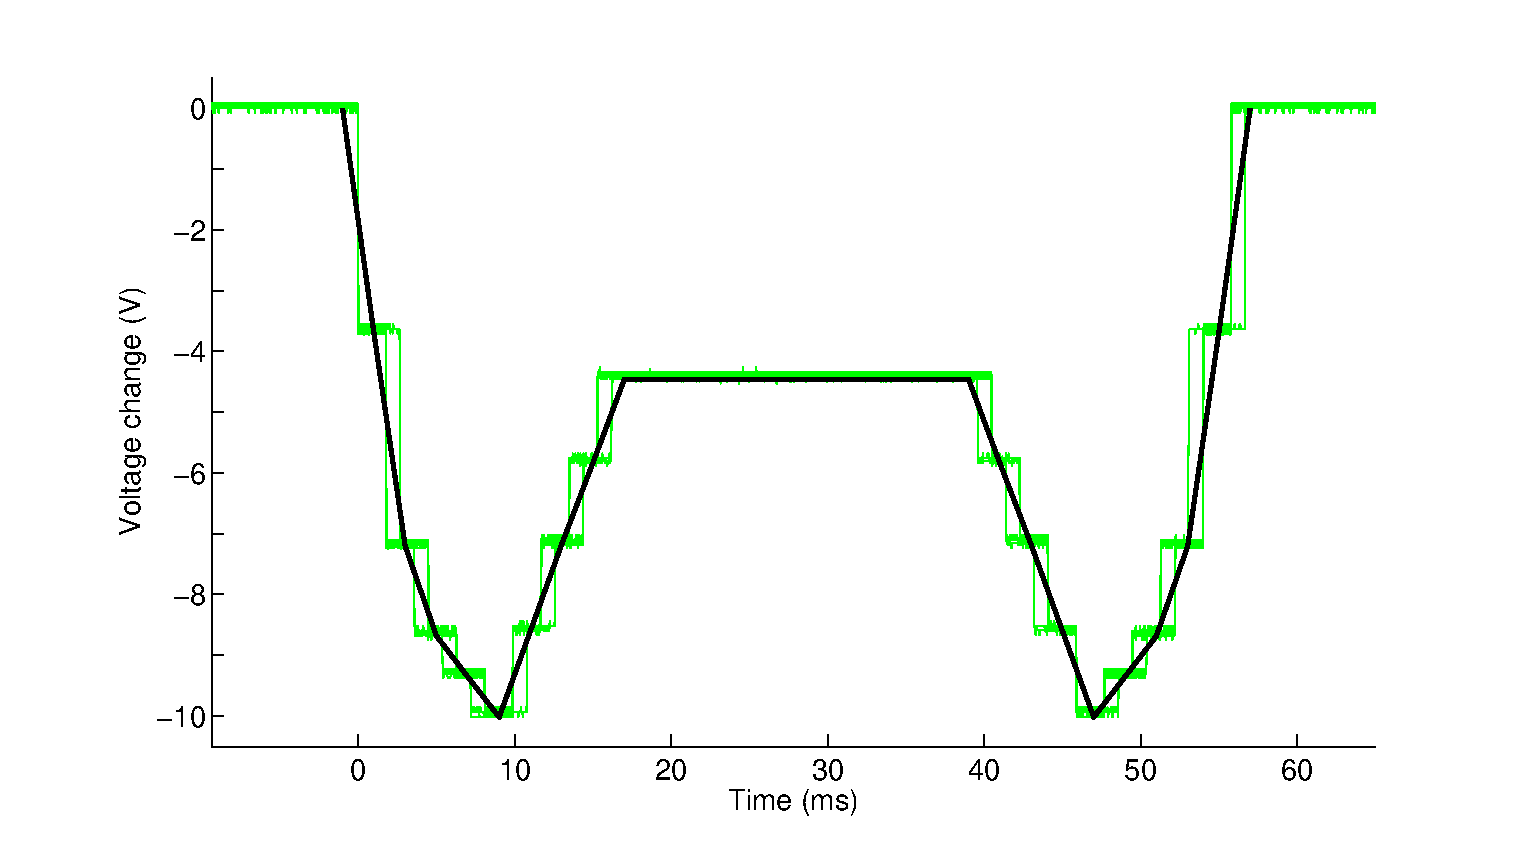
\includegraphics[width=14.5cm]{chapter7/waveform/rtusual/rtusual}
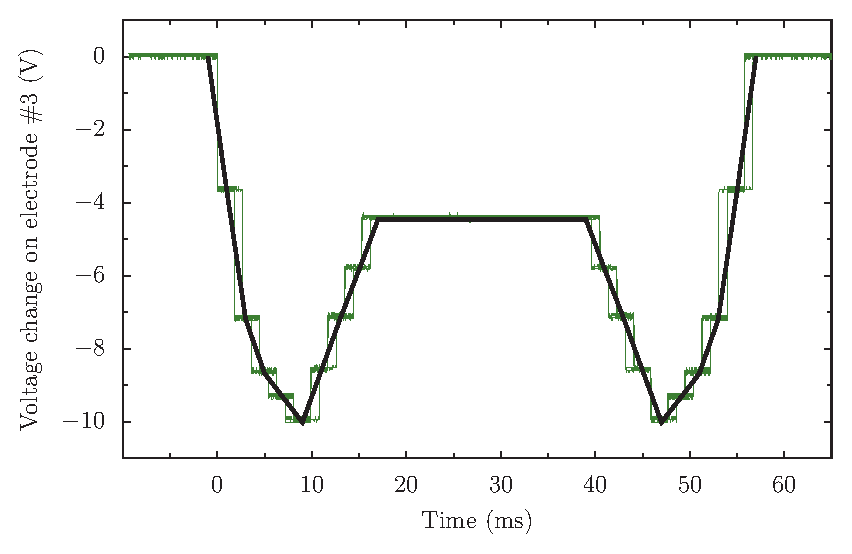
\includegraphics{chapter7/waveform/rtusual/recordedwaveform_v1}
\caption[Example of recorded waveform for ion shuttle]{Example of recorded waveform for electrode pairs \#3. The solid line connects the set voltages; update rate is 1/\ms. The voltages were recorded by an oscilloscope, and 20 repeats are plotted.}
\label{fig:rtscopewaveform}
\end{figure} 

% 
% \begin{figure}[h!t]
% \centering
% 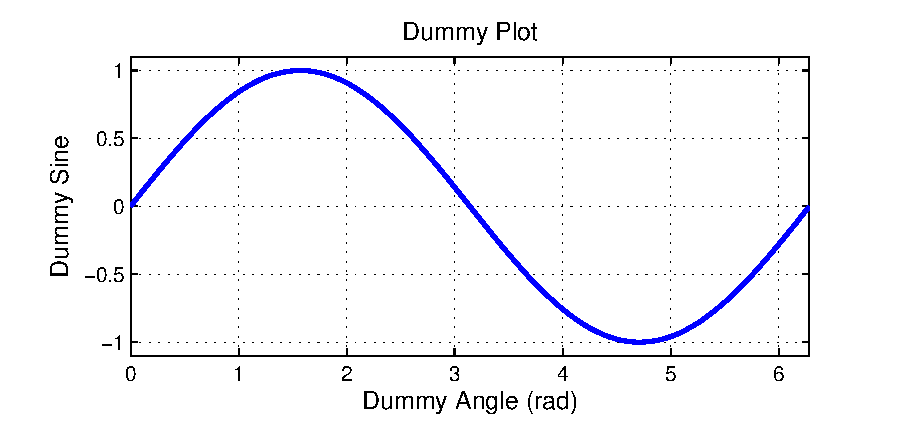
\includegraphics[width=8cm]{dummy}
% \caption[]{}
% \label{dummy}
% \end{figure} 
